\documentclass[a4paper,man,natbib,floatsintext,import]{apa6}

\usepackage{longtable}
\usepackage[english]{babel}
\usepackage[table]{xcolor}
\usepackage{lscape}
\usepackage[utf8x]{inputenc}
\usepackage{amsmath}
\usepackage{graphicx}
\usepackage[colorinlistoftodos]{todonotes}
\usepackage{pdfpages}

\title{Analogical Transfer in a Hebb Repetition Paradigm}
\author{Oesch Adrian}
\affiliation{University of Zurich}
\shorttitle{Analogical Transfer in a Hebb Repetition Paradigm}
\begin{document}

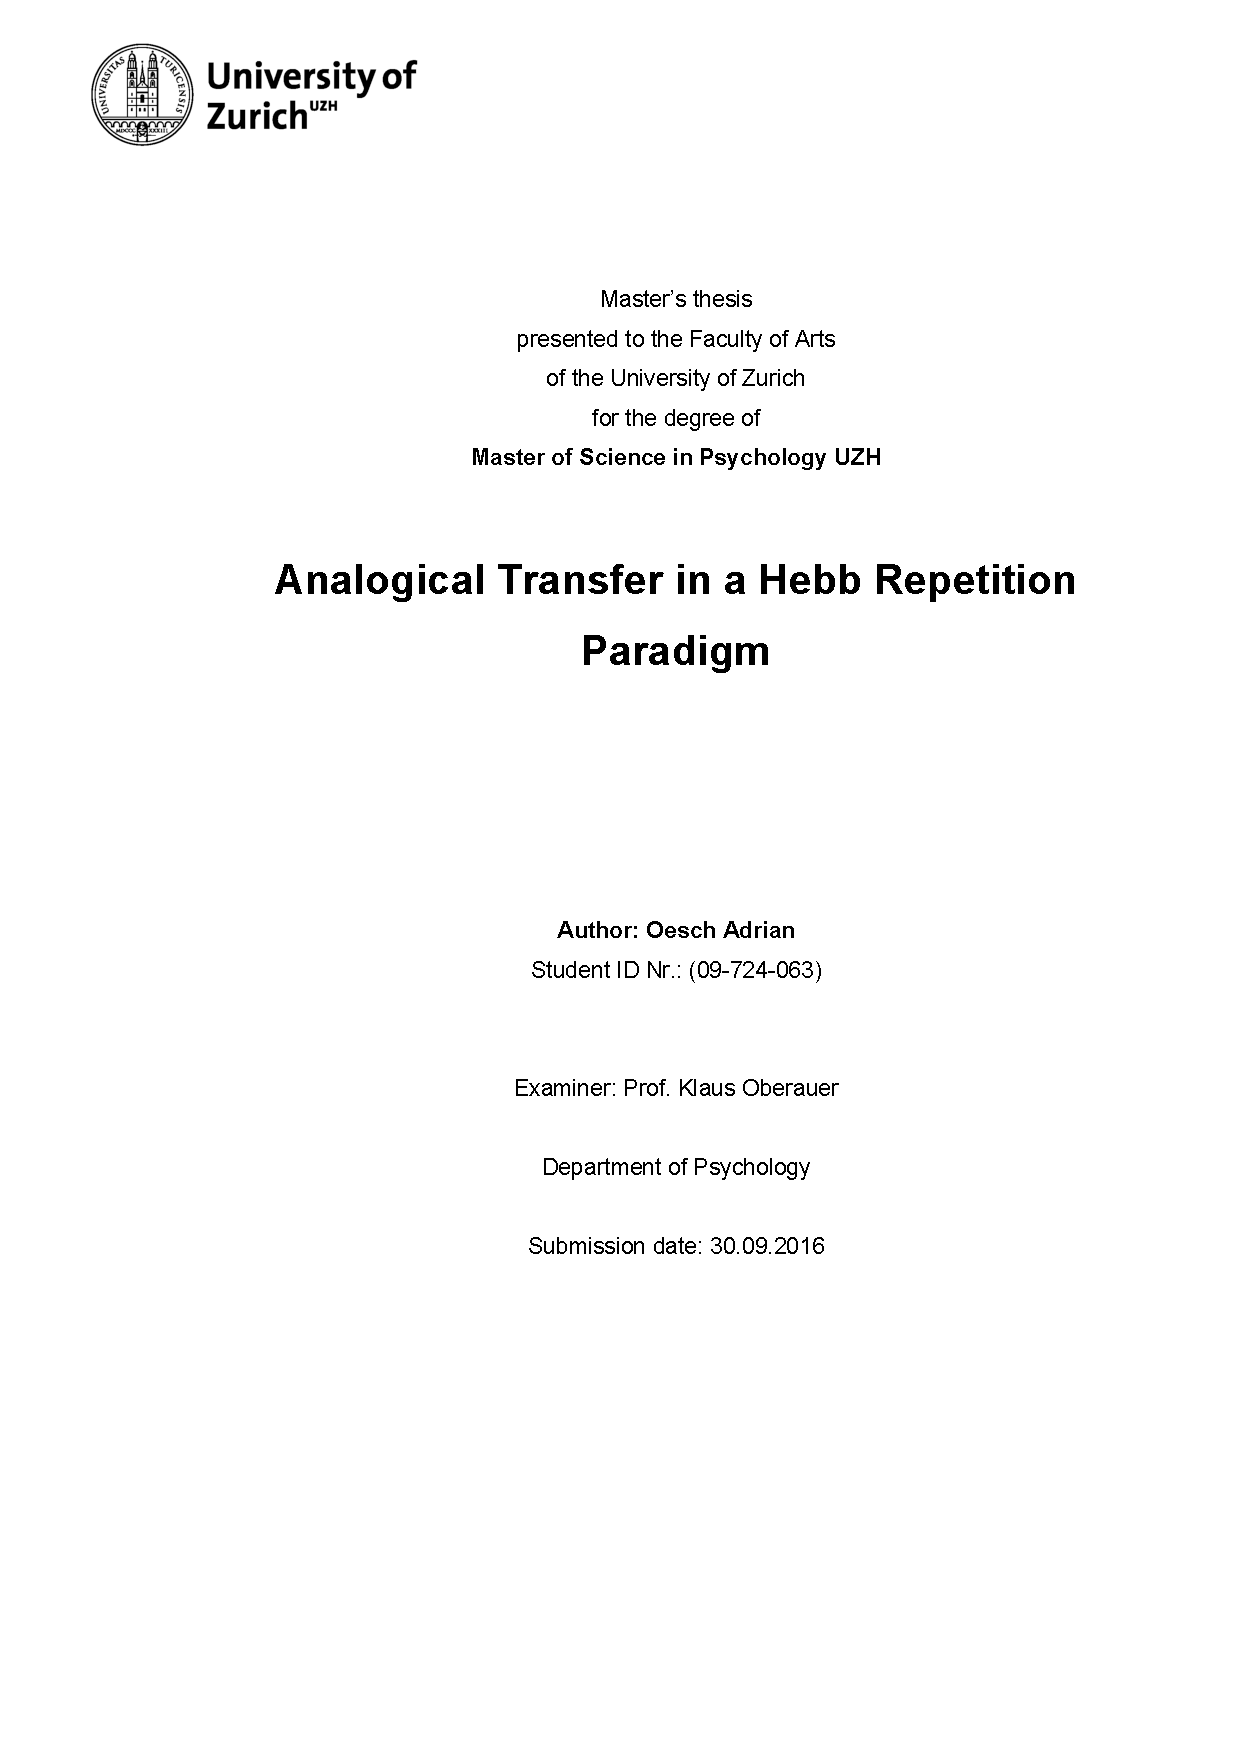
\includepdf{cover}
\section*{Abstract}
Previous research has shown that participants unintentionally map analogical word pairs on to each other due to relational similarity \citep{Popov2015,Estes2006}. Also, it has been discovered that structural similarity guides analogical retrieval in reminding studies \citep{Wharton1996}. This thesis aims to combine those lines of research and investigates unintentional analogical transfer on the basis of mere structural similarity. By combining the Hebb repetition paradigm with original story material, a novel experimental setting was developed to investigate this hypothesis and contribute to growing evidence that analogical transfer is not a deliberative reasoning process, but happens also unintentionally. Weak evidence (5\%-sign. level) for this hypothesis was obtained in experiment 1, where an increased recall performance over trial index in stories with high structural similarity was observed. This effect could not be replicated in experiment 2, where a limited reading time was introduced.

\newpage
\tableofcontents
%\listoftables
%\listoffigures

\newpage
\section{Introduction}
\subsection{Analogy: What is it good for?}
Recently I was listening to a podcast about economics where an expert compared money to blood. He explained that when our economy would be our body, then the blood would be the money and the heart would be the financial sector distributing the blood around the body. I immediately felt I had a better understanding of why money and banks are relevant to our financial system.
This is a typical example of an analogy. Through the alignment of entities of a less known system to the entities of a better known system, I started attaching the unknown to the known. Every analogy has two models: a source and a target model. The expert uses the information from the better known model, i.e. the blood system in the previous example, in order to explain the value of the monetary system. Thus, the blood model is the source and the monetary system is the target. The process of alignment is called mapping. In a well matching analogy every element of the source model has a counterpart in the target model. Blood gets mapped on to money and the heart on to the financial system. I already knew that the heart allocates the necessary resources to different organs by pushing blood throughout the body. Because we can map those relations from the target on to the source and their corresponding entities, this process is also called analogical transfer. The more entities and relations of two models match on to each other, the higher the systematicity of an analogy is \citep{Gentner1997}. I can try to align more elements to increase the systematicity of our previous example: If blood is money and the heart is the financial sector, the organs might be different industries. Each industry/organ has a different function, but still all of them rely on having a sufficient blood/financial supply. Also, the higher the blood supply of an organ is, the more energy it can use. Similarly, a higher blood supply could be mapped on to higher investment opportunities in some industries than in others in the financial model. The brain for example uses a lot more oxygen and therefore needs a higher blood supply. Analogically one could say that the insurance industry is a finance heavy sector and is equally important to an economy as the brain is to the body. We have hereby increased the systematicity of this analogy, because the mapped systems grew bigger and more elements could be matched on to each other. But this alignment process can also be stretched too far and mapping opportunities have limits: If blood is money, what then is the oxygen in the blood regarding the financial sector? Generally people tend to prefer analogies with higher systematicity for inference as the coherence and soundness of the comparison is increased \citep{Clement1991}.

Due to its powerful applications analogies can be found in numerous professional domains. An often cited example within the realm of schools and education is the comparison of electricity to the flow of fluids that teachers use to explain new concepts like voltage in science class \citep{Treagust1992,Dupin1989,Gentner1982}. Other researchers have investigated analogies in politics. It was expedient for president Bush Sr. to compare Saddam Hussein to Adolf Hitler when entering the war in Kuwait in 1991, because he wanted the attributes from Hitler to be also attributed to Saddam Hussein \citep{MacDonald2002}. Analogies are also common in other situations of persuasion like in marketing \citep{Herzenstein2014,Cornelissen2003} and they are also considered to be very important in the innovative process in science, research and development \citep{Gentner2002}. \cite{Dunbar2001} found out that scientists heavily rely on analogies in lab meetings. Yet another impressive feature of analogies is that knowledge that was acquired through analogical comparison is used more frequently in similar subsequent tasks, than if the same material is just summerised \citep{Gentner2003a,Loewenstein1999}. Also, the Ravens Matrices Test, which relies on analogical reasoning, is one of the common standard tests to measure general intelligence \citep{Carpenter1990}.

Apart from systematicity, analogies can also differ regarding the level of similarity. Comparing a story with dogs to a story with cats is a close analogy, because both animals share a lot of surface features like the number of legs, the tail, the fur, the way of moving and so on. But comparing a story with a dog to a story with humans, one has to focus on relations in order to detect similarities. Dogs and humans only share little salient features that make them comparable to each other. Only by considering the entities in relation to other entities we can detect similarities. When for example a bitch is watching out for her offspring, we can draw a parallel to a woman taking care of her child. This comparison is based on the similar relation between the entities, e.g. "watching out for" and "taking care of someone". Through this more abstract level of similarity, we can also map the entities on to each other. Without any kind of similarity, it is not possible to map models on to each other, because no entities and relations can be aligned.
Remote analogies or true analogies \citep{Wharton1996} - the mapping of models with no or only little surface similarity - are the most challenging analogies because they rely on an even more abstract level of similarity: structural similarity or higher order relational similarity \citep{Catrambone2002} (examples will follow). Detecting remote analogies can be especially advantageous in problem solving situations, when search strategies based on surface features have not triggered a detection of a suitable solution. One can also think of it as an expansion of the search space. By relying on abstract features, the amount of potential candidates for comparison increases a lot.

\subsection{Analogical Transfer and Problem Solving}
In a famous experiment \cite{Gick1980} first presented the participants three stories. They had to first memorize those stories and recall the content of each story as precisely as possible. One of those stories was about an army general who wanted to invade a fortress. The general knew that if his army reached the fortress, his force would be big enough to capture it, but there was a problem. The army couldn't simply march towards the fortress, because the road leading to the fortress was mined and only small groups could safely pass it. The solution to the general's problem was to split his army into multiple smaller forces, which he then let simultaneously march on multiple roads from different directions onto the fortress. That way the many small groups could pass the mined roads and rejoin forces at the fortress, to then attack and conquer it. This is also called an attack-dispersion solution. The other two stories served as distractors and were as nonanalogical as possible to the general story but similar in length.

After all stories were memorized, recalled and a short break, participants were confronted with a new a problem solving task: a doctor has a patient with a tumor in his stomach. The patient can't be operated and thus is going to die unless the tumor is removed. The doctor could make use of rays, which might destroy the tumor when intense enough, but they would also damage the healthy tissue on the way to the tumor. At lower intensity, the rays don't damage the healthy tissue but neither the tumor. The solution to the doctor's problem is to apply the attack-dispersion schema like in the story with the general: split the bundled force into multiple weaker ones, and only join the forces together where it is necessary. This inference from one story to the other can only be transferred if the participant detects the similarity between the general's and the doctor's problem. Rays don't look like an army, and a fortress shares only very few features with a tumor, therefore it can be argued that only structural similarity can be the foundation of this analogy.

The way the two stories are presented in the previous paragraph makes the analogy evident and easy to detect. But in the experiment by \cite{Gick1980} only 21\% of participants in the group without a hint came up with the dispersion solution, versus 91 \% in the group with a hint. \cite{Gick1983} replicated the solution rates in various slight modifications of this experiment, leaving the question open: why is it that hard to detect similarities between systems based on structural similarity? Why do spontanous remote analogies, the main focus of this thesis, occur relatively rarely?

\cite{Gick1980} argues that memory might be sensitive to the encoding context. In the first experimental phase the story material was encoded in the context of a memorization task, while later they were confronted with a problem solution task. Why should anyone assume those tasks have anything in common and therefore relate the content of both tasks to each other? Also, they further argue that analogical retrieval might be sensitive to the semantic context of the target story in problem solving tasks. Why should one be reminded of a general when trying to solve a doctors problem? One could just as well think of farmers or teachers. They share about the same features (surface similarity) with the doctor as with the general. Various experiments showed that analogical retrieval is much more likely when the source and target models have similarities on lower levels of similarity i.e. the surface \citep{Gentner1993,Holyoak1987}.

\subsection{Unintentional Analogical Processes}
In contrast to the line of research provided in problem solving paradigms, more recent studies have started to investigate analogical processes that happen on an much more frequent basis. While in the standard problem solving paradigm spontaneous analogical transfer only rarely occurs, studies involving relational priming investigate whether analogical processes might be effective in much more general cognitive processes. Priming studies have been widely used to study semantic memory throughout the second half of the 20th century \citep{Lucas2000}, but rarely have they focused on the relations between objects. Processing of relations between objects is crucial to the mapping process in remote analogies, because the detection of similarity between two remote systems can only rely on structural similarity. Relations between objects can be viewed as a first level of abstraction \citep{Catrambone2002}. \cite{Spellman2001} conducted one of the early relational priming studies. They found that participants were faster in lexical decision tasks when the same relation was implied but not explicitly mentioned by a previous pair of words, but only when participants were instructed to note and use the relations. The effect was not observed when subjects were merely reading the word pairs. It has been argued, that those effects were mere side-effects from associative priming \citep{Gagne2005}, but \cite{Estes2006} presented evidence, that this is not the case, by controlling for lexical similarity independently from relational similarity.

\cite{Hristova2009b} additionally could show that relational priming is also present in a color naming paradigm with pairs of words, where one word per pair changed its color 1'000 milliseconds after appearance. When the prime word pair was in green and the cue word pair also turned green, therefore the colors were congruent to each other, then the participants reaction times were faster when those two word pairs were analogical, suggesting that an unintentional mapping process facilitates the color naming process in congruent color situations, resulting in shorter reaction times, even though people were not asked to relate the content of the word pairs to each other.

\cite{Day2007} applied a different experimental setting to uncover unintentional analogical processes. In this study participants had to read two stories. After the second story, they were asked a few questions, which were not clearly answerable from the previous story itself. While both groups read the same second story, the groups were reading different analogical first stories. The two groups differed significantly in terms of how they interpreted the second story, depending on which story they had read first. They were not instructed to infer from the first story, and when asked in a post-experiment survey, almost 80-\% of participants were responding, that they felt that the stories were understandable on their own and that they answered the questions without inference from other stories. In addition to this finding, the participants also encoded the target statements in the second story faster, if the statements were structurally similar to the source statements of the first story.

These experiments go along with a line of theorizing, which views analogy making as a much more fundamental cognitive process than deliberative reasoning. \cite{Chalmers1992} describe analogical reasoning as kind of a high level perception. Their theory proposes a universal process of information aggregation throughout different levels of perception. Remote analogies, the main topic of this thesis, might be only be the tip of the iceberg because it's the most abstract, but according to \cite{Chalmers1992}, relies on the same processes as lower level processes like object recognition or concept formation. Also, \cite{Hofstadter2001} argues that analogical reasoning is the actual core of cognition, "for without concepts there can be no thought, and without analogies there can be no concepts" \citep[p. 34]{Hofstadter2013}. The role of analogies as a fundamental cognitive process has already been expressed by other researchers as well. While using a different terminology \cite{Kokinov1994} developed a model he called "Associative Memory-Based Reasoning" where he tried to connect analogical reasoning literature to other streams of cognition research. Others argue, that relational priming is the basis of analogical access, relying mainly on research from developmental psychology \citep{Leech2008}.

Now so far various experiments show that spontaneous analogical transfer based on structural similarity is rare, while at the same time it has been shown, that analogical models are also being unintentionally mapped on to each other on the foundation of mere relational similarity. Taking the current state of research regarding unintentional analogical transfer one step further, this thesis aims to find evidence for unintentional analogical transfer on the foundation of mere structural similarity, increasing the foundation of the mapping process to a higher level of abstraction.

\subsection{Structural Similarity and Analogical Access}
\cite{Holyoak1987}, \cite{Johnson1992} and \cite{Wharton1996} presented evidence that structural similarity has an effect on analogical reminding. In the experiments by \cite{Wharton1996} participants were asked to read a set of target stories first. After a certain time, which they varied across experiments, the participants were asked to read another set of cue stories. Each of those cue stories had either one or two potential target candidates, depending on the condition double target or single target. They varied the relations between cue and target stories according to two factors: surface similarity and structural similarity (they used situational similarity and thematic similarity for those terms). In the double target condition both target stories were either remote or close, but differed in their structural similarity. Figure \ref{fig:wharton} depicts the result of this study. At first, one can detect a clear difference between close and remote cue stories, confirming previous experiments on the significance of shared low order features. But when comparing the analogical to the nonanalogical cue stories, those experiments also indicate an effect of structural similarity on analogical reminding, therefore the authors conclude that structural information does guide analogical reminding. The authors although emphasize that reminding doesn't necessarily lead to analogical retrieval, as the instructions in a reminding paradigm differ crucially.

\begin{figure}
\centering
\begin{minipage}[t]{0.5\textwidth}
\fitfigure{figures/wharton_96.png}
\caption{Reminding frequencies from \cite{Wharton1996} for both close/remote (surface similarity) and analog/disanalog stories (structural similarity).}
\label{fig:wharton}
\end{minipage}
\end{figure}



\subsection{Hebb Repetition Paradigm}
To test the hypothesis whether structural similarity suffices for unintentional analogical transfer, an experimental paradigm from memory research was applied. The Hebb repetition paradigm was first introduced by Donald Hebb in 1963 \citep{Lafond2010}. He presented participants sequences of digits and asked participants to recall the items of those sequences in order of appearance after each sequence. This task is also called serial recall. One sequence of digits, the target sequence, was repeated every third trial. The other sequences in between of the target sequence, the filler sequences, were all different from each other. The Hebb repetition effect describes the increase in recall performance over repeated presentations of the target sequence compared to the filler sequences. This effect has been studied since its introduction in numerous ways with variations regarding the size of the sequence, the content of the sequence, the amount of filler sequences between the target sequence and complexity of the task \citep{Lafond2010,Oberauer2015}. \cite{McKelvie1987} detected that the effect is also present if participants are not noticing the repetition of the target sequence.
Hebb and other researchers saw this experimental paradigm as a model of long term learning because the effects of increased memory performance on the target list often lasted a long time. Due to the thorough investigations of this effect and robust results, I think the Hebb repetition paradigm is a suitable candidate, to test our hypotheses. Instead of presenting sequences of digits, I constructed two pools of stories: A pool with analogical stories, which all share the same causal structure. These stories with a common causal structure serve as the target stories, while the pool with nonanalogical stories, which don't share a causal structure, are equivalent to the filler sequences in the Hebb repetition paradigm. The Hebb repetition paradigm relies on improved access to information through repeated activation of a sequence. Analogical to the classic Hebb repetition paradigm, I predict an increased memory performance in analogical stories through repeated activation of the same causal structure in analogical stories compared to nonanalogical stories. This implies that participants will have increasingly more resources available to remember other elements of the stories than the causal structure in analogical stories, because the causal structure stays the same. In contrast to priming studies, where it could be shown that the activation of a relation, affects the processing of a subsequent similar relation, a specific relation usually can only be activated once. The possibility of repeated activation of the same abstract structure in this setting, seems to make it an especially well suited method to show subtle effects.

\newpage
\section{Experiment 1}
\subsection{Methods}
To test those hypotheses a novel task was developed, where participants had to read different stories consisting of a sequence of statements and recall the content of those statements in order of appearance after each story. All stories differed on the level of the surface, meaning that the semantic context of the story differed between all stories and the amount of shared surface features should be kept at a minimum. Every second story had an analogical story structure, resulting in a sequence of alternating analogical and filler stories. A pilot study investigating an ideal amount of statements per story, so that the task to recall wasn't too difficult on the one hand, and the task to come up with suitable stories neither on the other hand, led me to the conclusion to use stories with three statements.
All experiment material source code is available on Github \citep{Oesch2016}.

\begin{figure}
\begin{center}
\fitfigure{figures/example_response_menu.png}
\caption{Example of a response display for the statement "Mining company Ahow has a lot of resource Pishi."}
\label{fig:example_response_menu}
\end{center}
\end{figure}

\begin{figure}
\begin{center}
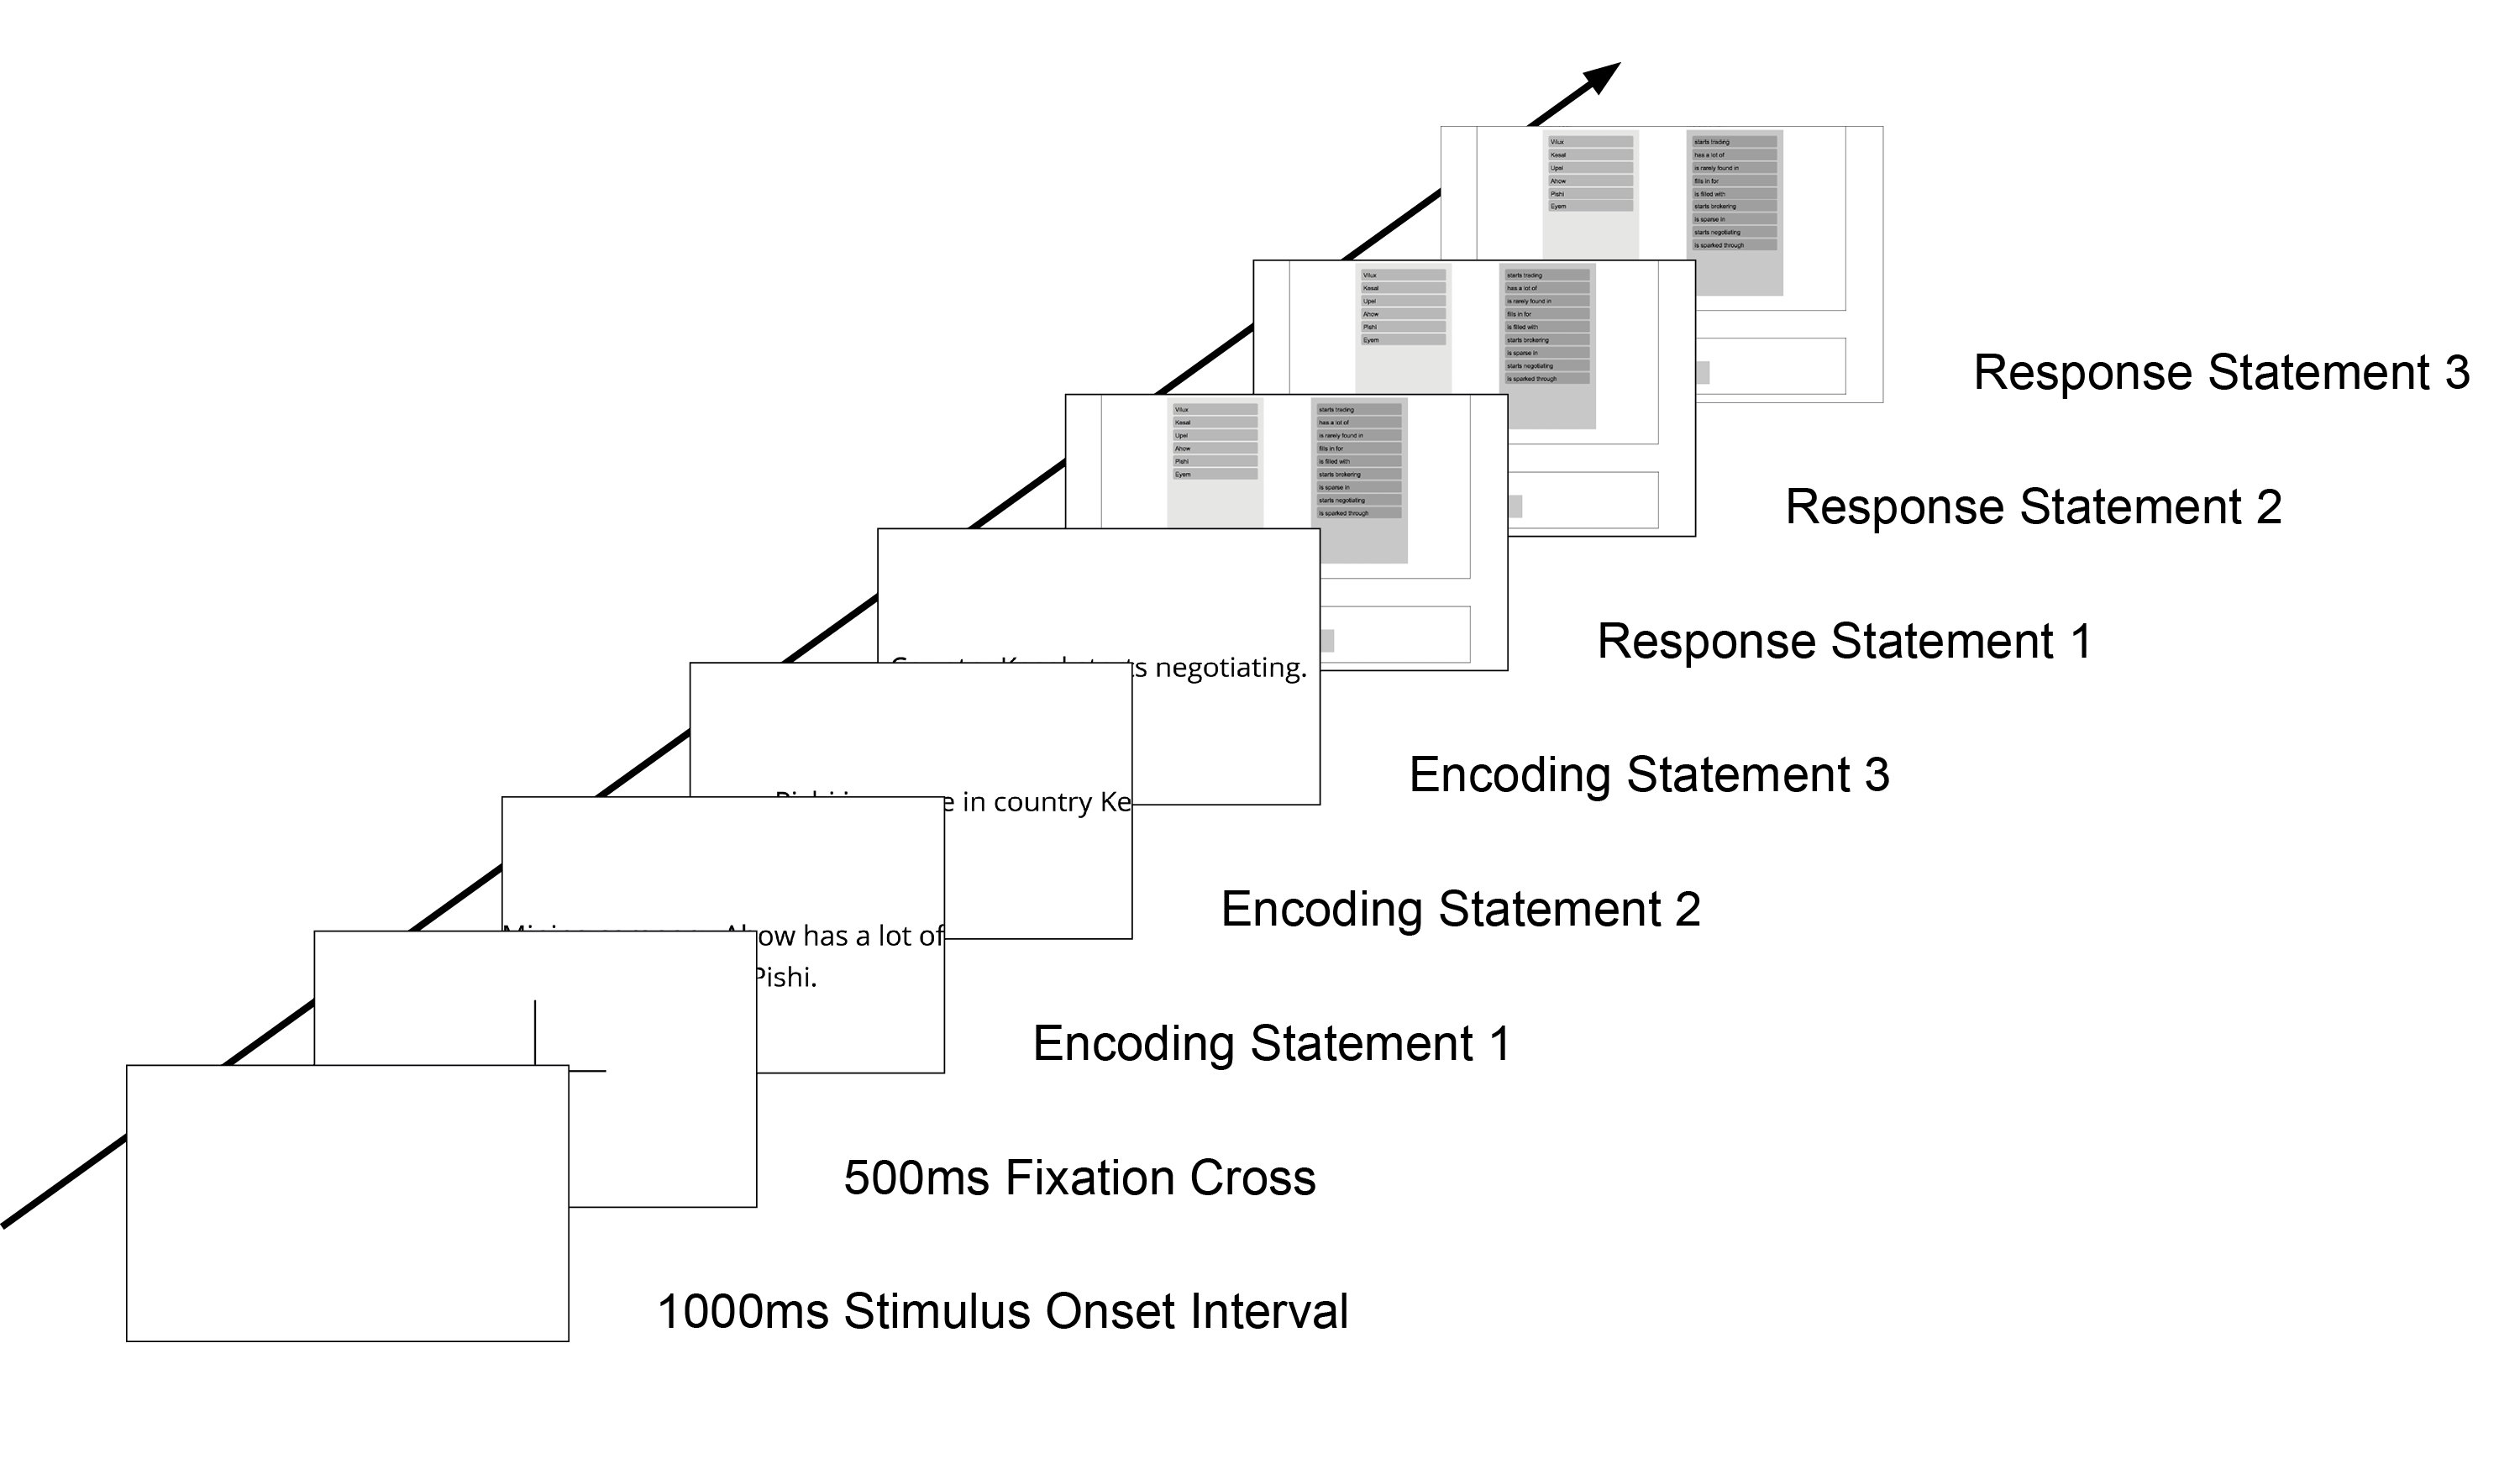
\includegraphics[width=\textwidth]{figures/trial_sequence.png}
\caption{Sequence of a single trial.}
\label{fig:trial_sequence}
\end{center}
\end{figure}

\subsubsection{Participants}
For data collection I collected 109 observations from the online labour platform CrowdFlower. In the description of the task on CrowdFlower I explicitly asked for native english speaker, and set the country parameter on CrowdFlower to United States only. Nonetheless 4 participants responded with different native languages than english in our post experiment survey and were therefore excluded from further analysis. In addition, 17 participants didn't pass the trick story to assure participants were paying attention and where they were supposed to recall a single statement (2 names and one relation) and where the response options offered 2 names and 3 relations. Those subjects were also excluded, which resulted in a sample of 85 subjects. Figure \ref{fig:sample_age} shows the sample's age distribution which varied between between 20 and 65 years old (median at 37), a rather wide age spectrum compared to traditional college student samples. The sample was equally distributed in terms of gender (50.3\% female). According to the self-reported highest degree of education, most of our sample had a university/college degree (58\%). Fewer had a high-school degree (39\%), and three subjects (3.6\%) reported having a doctoral degree.

\begin{figure}
\begin{minipage}[t]{0.5\textwidth}
  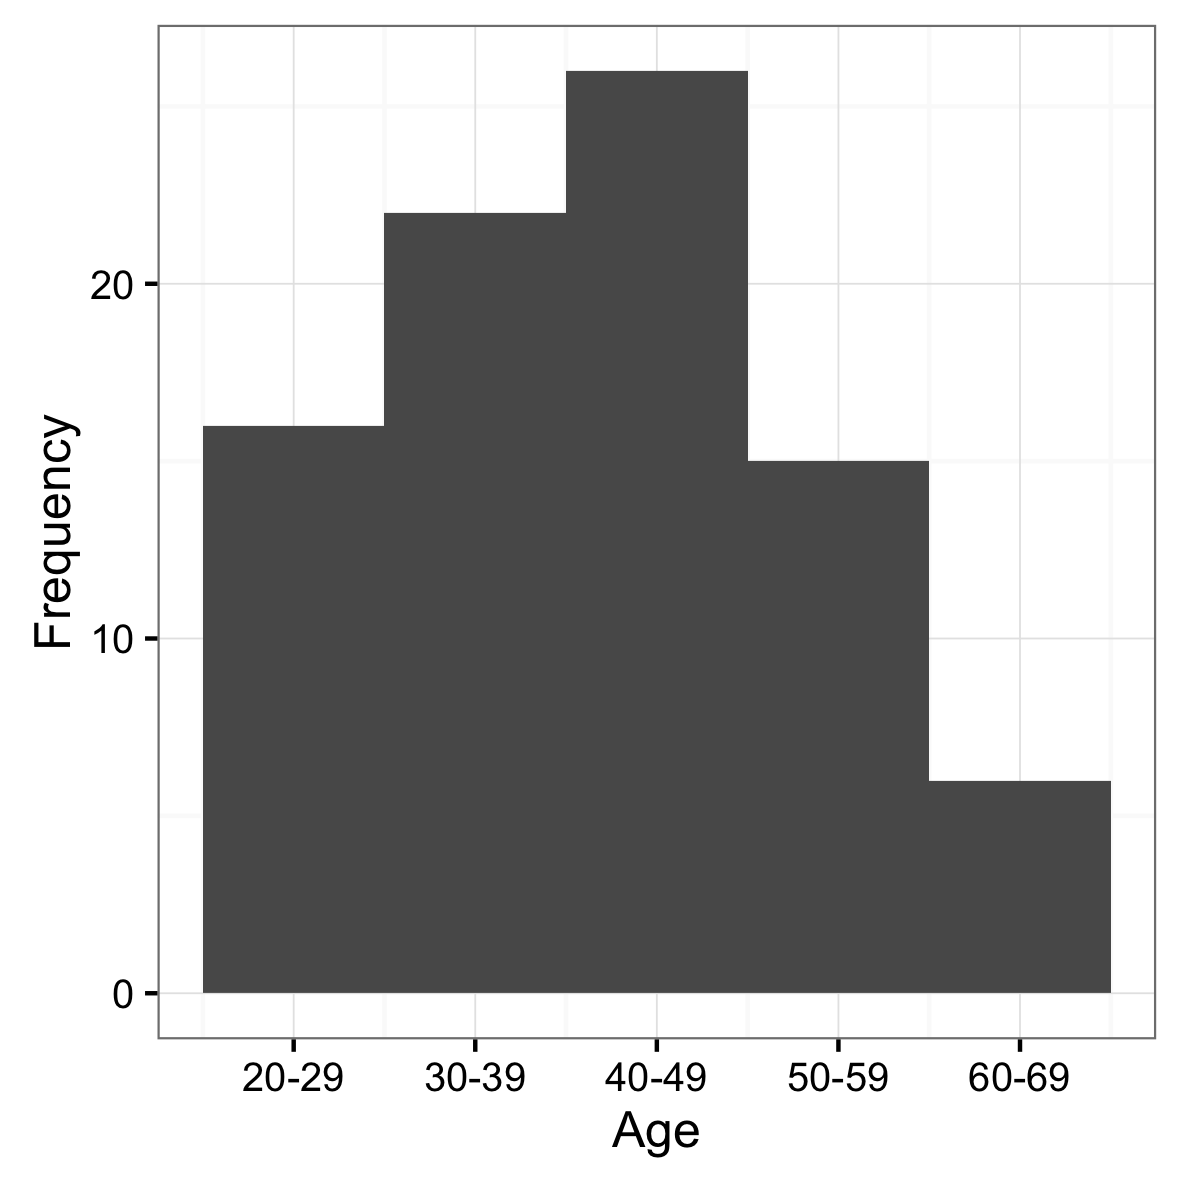
\includegraphics[width=.9\linewidth]{figures/sample_age.png}
  \caption{Distribution of age in the sample of experiment 1.}
  \label{fig:sample_age}
\end{minipage}
\begin{minipage}[t]{0.5\textwidth}
  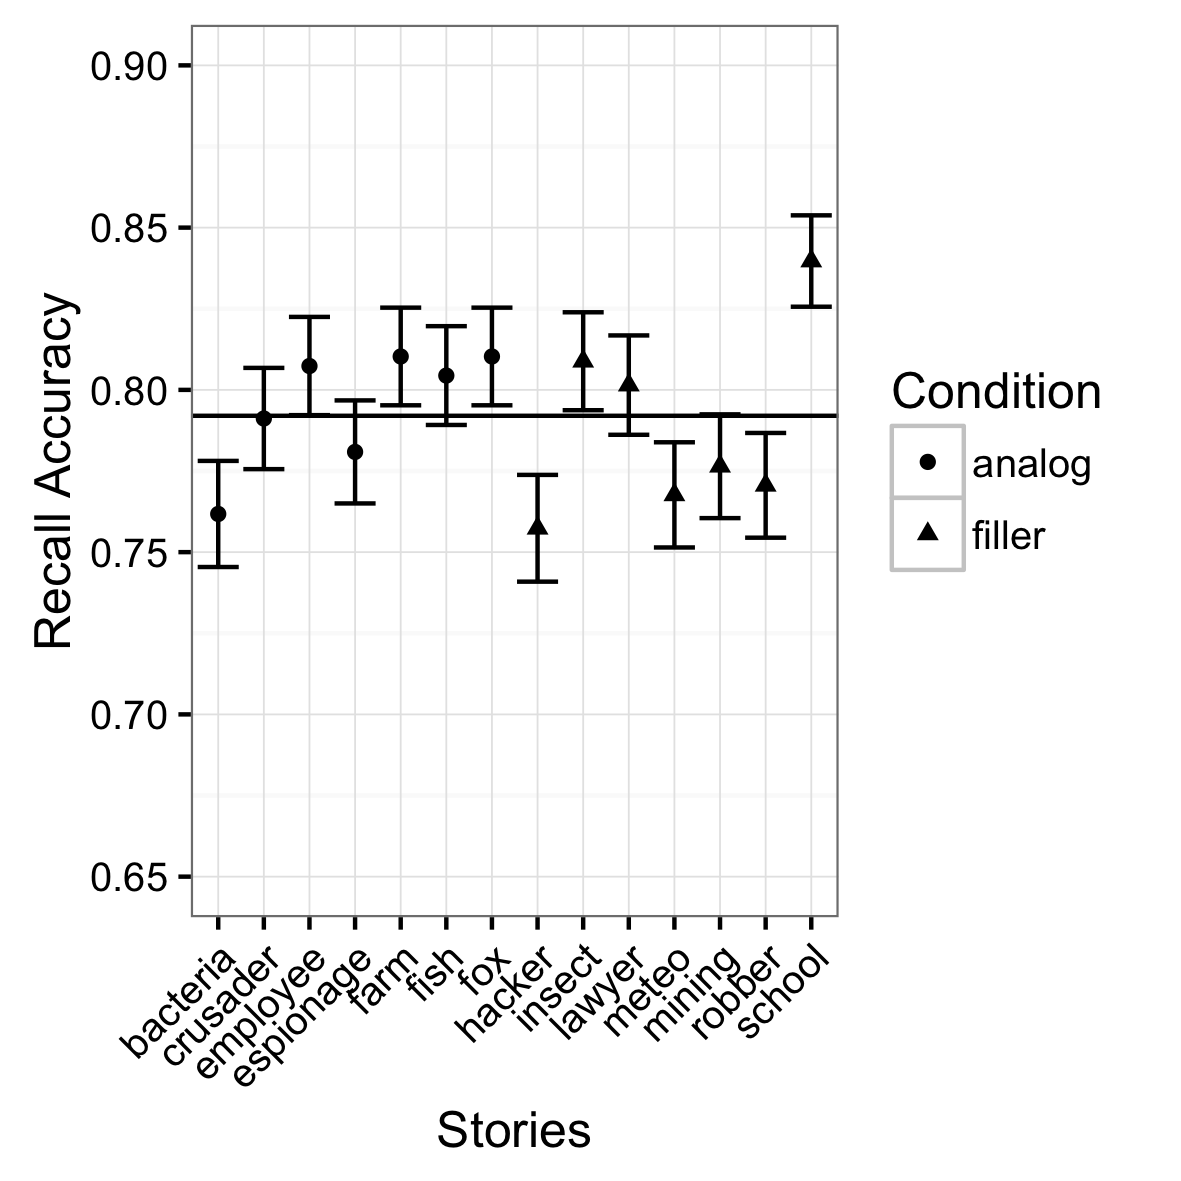
\includegraphics[width=.9\linewidth]{figures/material_stories.png}
  \caption{Mean recall accuracy and standard error for each story plus grand mean.}
  \label{fig:material_stories}
\end{minipage}
\end{figure}

\subsubsection{Material}
For the purpose of illustration I want to present two examples of analogical stories first: (1) "Hacker Uhuy wrote computer code Wehif. Code Wehif cracks the firewall of company Thisun. Company Thisun suffers a data loss." and (2) "Bacteria Yuxeh emits enzyme Afi. Enzyme Afi dissolves the membrane of organ Eshov. Organ Eshov fails." Also, an exemplary filler story: (3) "Cloud Vuloz collects humidity over ocean Matmag. Ocean Matmag lies next to the beaches of area Ofes. Area Ofes is fertile."
I constructed two sets of short analogical and filler stories consisting of three statements each. The goal was to build all stories with a minimum of surface similarity overlap, i.e. no two stories with animals or where plumbers have a lead role. In the examples above the context changes from Hackers to Bacteria to Clouds, which I assume to have about an equal low amount of surface features in common. The first two statements each have the structure: entity, relation, entity. The last statements only consisted of an entity followed by a relation, which represented a conclusion from the two previous statements. Three named entities were part of each story.  To rule out individual differences in name recognition, and also to make the task more difficult, the names of the entities were randomly constructed by a free online service on dialectcreator.com so they were nonsensical. All analogical stories had the following causal structure: "Entity A is responsible for entity B", "Entity B overcomes protection of entity C" and "Entity C endures negative consequence". If we compare example 1 and 2 from above, then we can clearly see, that we can map all the relations and entities onto each other. We can align the Hacker who writes a computer code to overcome the firewall of a company, with the bacteria which emits an enzyme to dissolve the membrane of an organ. While it is not sound to map Cloud Vuloz (3) into the same causal structure. Cloud Vuloz is not responsible for ocean Matmag, and neither does Matmag overcome Protection of Ofes. The filler stories were constructed to be linguistically as similar as possible to the analogical stories. The second statement in the exemplary filler story follows a similar syntax like both second statements from the analogical stories. To see the full table of stories and names see the appendix.
As response options I offered another alternative for each name, resulting in a total of 6 name-options per story, while only 3 of those appeared in the presented statements. For each relation from a story, I constructed two alternative response options, one was supposed to be synonymous to the correct relation, and one which was syntactically congruent but not in terms of the meaning. For example to probe the memory access to the relation of the second statement in story 2 from above, I presented following options: "cracks sth. of", "penetrates sth. of". and "catches sth. of". While "penetrates sth. of" has a similar meaning to cracking, the third option is dissimilar but is equivalent syntactically. This approach resulted in a total of 9 relation options per story. For each story I recorded 3 relation responses, one for each statement, and 5 name responses, 2+2+1=5 per statement, resulting in 9 items per story. I constructed 7 analogical and 7 filler stories for this experiment. This gave us 85*14*8 = 9520 binary observations of recall success to analyze with.

\subsubsection{Procedure}
I set up an online experiment using free hosting resources on Openshift (http://www.openshift.com). To run the experiment in the browser the open source JavaScript library jsPsych \citep{DeLeeuw2015} was used, which was developed explicitly to conduct psychology experiments in the browser. Participants had to open a link on CrowdFlower where they were sent to a webpage on our server on Openshift. I asked them to shut all other programs so they weren't disturbed by notifications. They were also reminded to put themselves in a quiet environment and reduce distractions like noise to a minimum. The experiment then launched into fullscreen mode and after giving consent and reading the instructions, the memory task was started.
After the presentation of a fixation cross for 500ms, a story was presented statement by statement. Participants were free to choose when to continue to the next statement by a forward arrow key press, but they could not go backwards. I decided to opt for free reading time, to be able to check if a repeated analogical story structure might also have an effect on encoding, as was observed in \cite{Day2007}, or the reading time might also have an effect on recall success. I mention in the instructions to "read the statements thoroughly, but don't waste too much time". After each story, the participants were asked to recall the content of the story, again statement by statement by choosing the correct name of the entities and relation out of two separate menus (one menu for the names and one for the relations). Figure \ref{fig:example_response_menu} depicts an example of the response display. Participants could use drag and drop to reconstruct the statements with the correct items. They were allowed to use as many drag and drop moves as they want and did not have a time limit either when reading or reconstructing a statement. Figure \ref{fig:trial_sequence} illustrates the sequence of displays of a single story/trial.
Alternately seven analogical and filler stories were presented like this. The order within the analogical and filler stories was randomized. Participants either started with an analogical or a filler story, although I had to fix this part of randomization due to a bug after I started collecting data. Subjects starting with filler stories were therefore collected at another date. After the 12th story I injected a trick story consisting of only one statement and two names, to check if the participants were paying attention. As response options, only the two names which appeared in the previous statement and three relation options were presented. After the trick story, I resumed with alternating another set of analogical and filler stories.
Following the memory task, a set of three closed yes or no questions regarding people consciously noticed different aspects of repetition were asked for, with the options to explain in an open format if participants responded yes to the closed question. The questions built up on each other, each being a little more specific about the repeated causal structure than the previous one. The first one asked if participants noticed any similarities between the stories, while the second one asked for repetiting elements between the stories and the third question explicitly mentioned the repeated analog/causal structure. See the appendix for exact wording of the questions.
Thereafter a set of questions regarding the demographics (age, gender, highest degree of education, native language) followed. Additionally I asked for the amount of effort on a four point Likert scale ("0 - none" / "1 - a little bit" / "2 - quite some / "3 - a lot"). I also asked if they completed the experiment in a serious manner and I therefore should use their data for analysis. I promised to give them the regular payment independently of their answer to this question. For the exact wording of the instructions used on CrowdFlower and in the experiment please see the appendix or the raw material on Github \citep{Oesch2016}. At the end of the experiment, every participant got a confirmation code, which they had to paste back into the form on CrowdFlower. After completion of the task Participants were paid one dollar for going through the whole experiment and received a bonus of another two dollars if they showed effort. The median of total experiment duration was 21 mins. Due to continuous bug monitoring, data was collected over various dates.

\subsection{Results and Discussion}
The raw code of the scripts used for figures and analyses is online on Github \citep{Oesch2016}.

\subsubsection{Material Assessment}
Even though I tried each story to be equally difficult to recall, when dealing with language material it is hard to neutralize a bias introduced by language. Figure \ref{fig:material_stories} indicates a certain difference between the stories regarding their difficulty, which is confirmed in an analysis of variance on item level, F(13,9506) = 2.303, p=0.005. It is therefore important that I account for this bias in further analyses with random intercepts.

\subsubsection{General Task Performance}
General recall accuracy was much higher than expected. A pilot study investigating suitable story length resulted in overall recall accuracies around 60\%. Median of overall recall accuracy in this experiment was at 83\% and over 30\% of our participants had recalled more than 90\% of items correctly. Figure \ref{fig:genper_overall} depicts the distribution of overall recall accuracies per subject. I mentioned in the instructions, that no means to facilitate this task were allowed, in contrast to the pilot study, where I didn't emphasize this. Also, this time I incentivized subjects to put effort into the task so they will receive a bonus, which could have led subjects to cheat.

\begin{figure}
\begin{minipage}[t]{.5\textwidth}
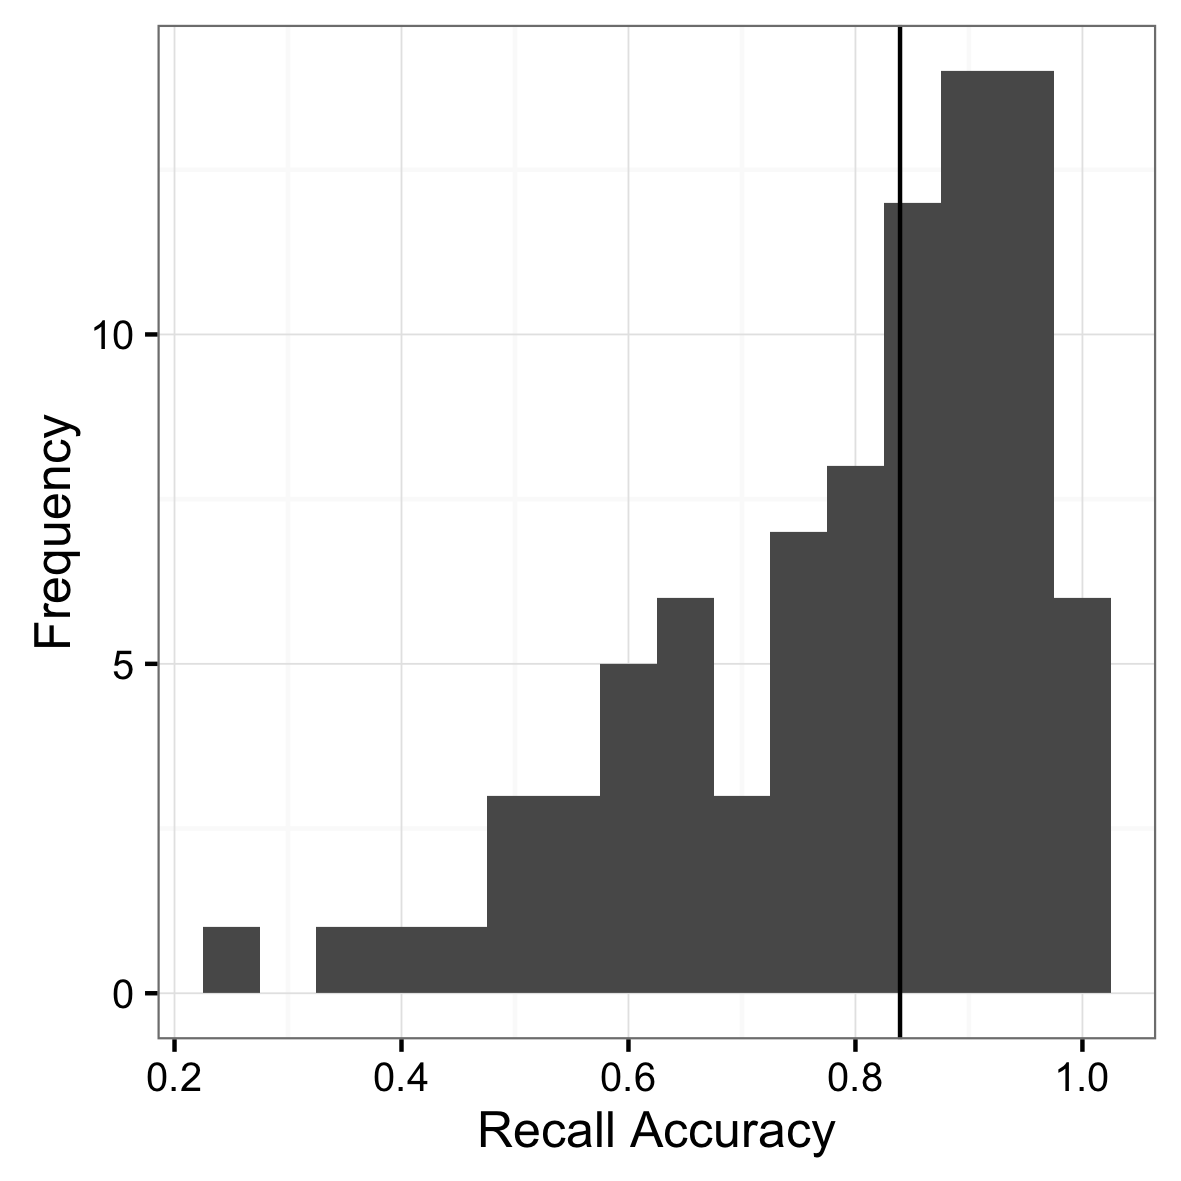
\includegraphics[width=.9\linewidth]{figures/genper_overall.png}
\caption{Distribution of overall recall accuracies per subject with median.}
\label{fig:genper_overall}
\end{minipage}
\begin{minipage}[t]{.5\textwidth}
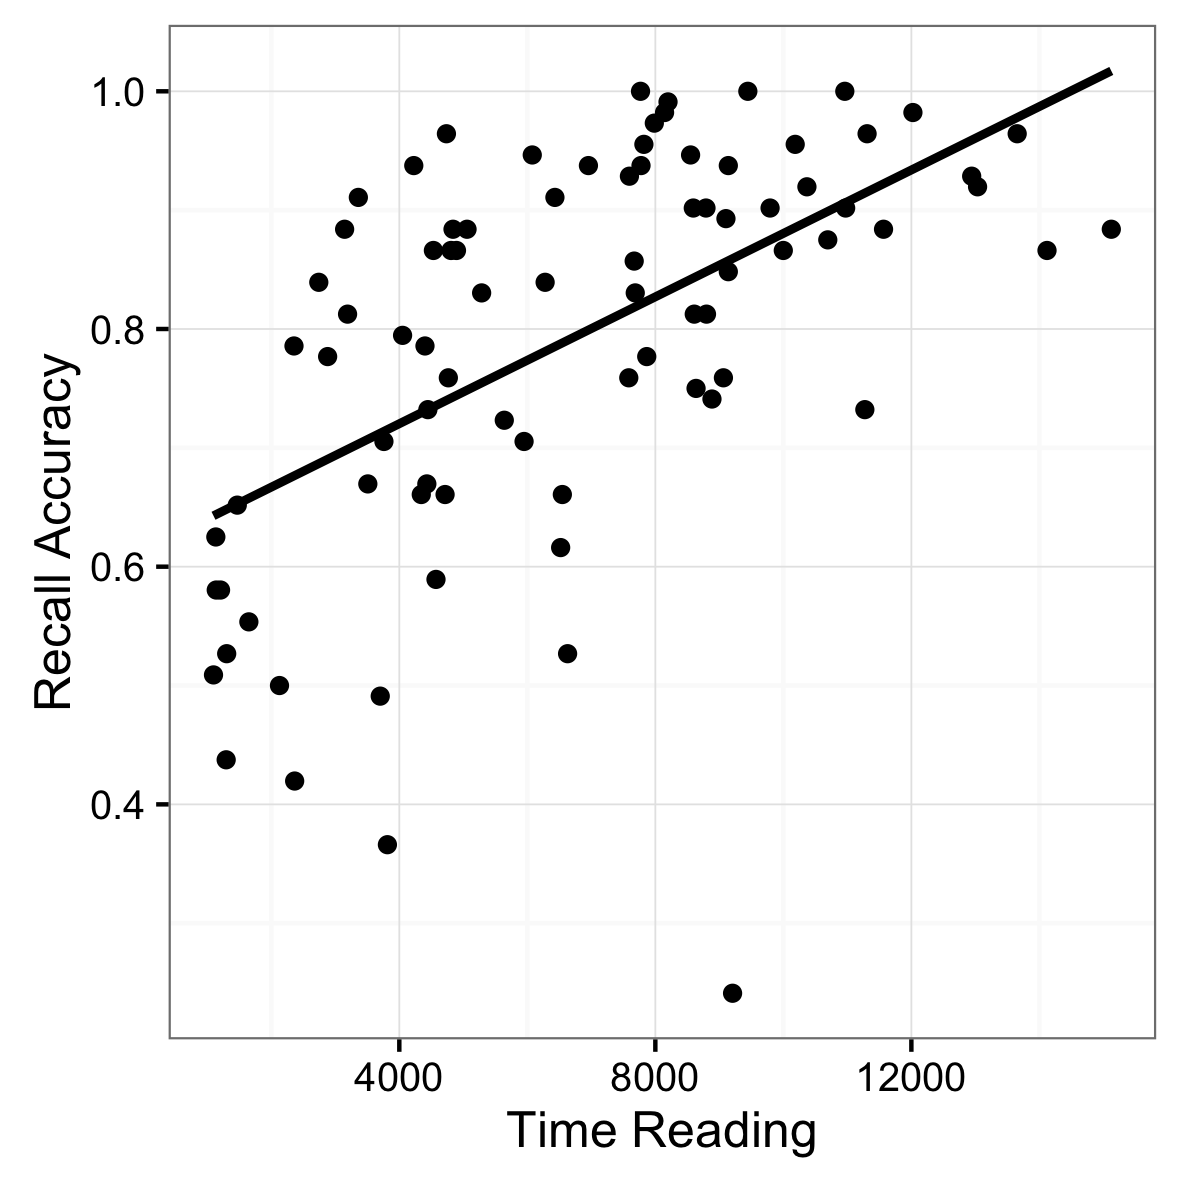
\includegraphics[width=.9\linewidth]{figures/genper_timeXoverall.png}
\caption{Correlation of subject's median statement reading time in milliseconds with overall recall accuracy.}
\label{fig:genper_timeXoverall}
\end{minipage}
\end{figure}


When comparing the median statement reading time per subject with the overall recall accuracies per subject (see Figure \ref{fig:genper_timeXoverall}), one can see an improved recall accuracy with increased median encoding time, the correlation is significant (\textit{r}(83) = 0.55, \textit{p} < 0.001). Half of our sample has a median of more than 6.5 seconds reading time for a single statement. This could be enough time to take notes (a little over 2 seconds per item), or just really put a lot of effort into encoding those two or three items and repeating the previous statement in a loop. Although comparing self reported effort with recall accuracies, there does not seem to be a big effect either (see figure \ref{fig:genper_effortXoverall}) and encoding time (see Figure \ref{fig:genper_effortXtime}). An analyis of variance with recall accuracy as dependent variable and effort as independent variable was not significant (\textit{F}(1,83) = 0.24, \textit{p} = 0.626). The ANOVA with the subject's median reading time was also not significant (\textit{F}(1,83) = 0.83, \textit{p} = 0.364).

% phonetic loop would also mean more reading time with increased statement length.

\begin{figure}
\begin{minipage}[t]{.5\textwidth}
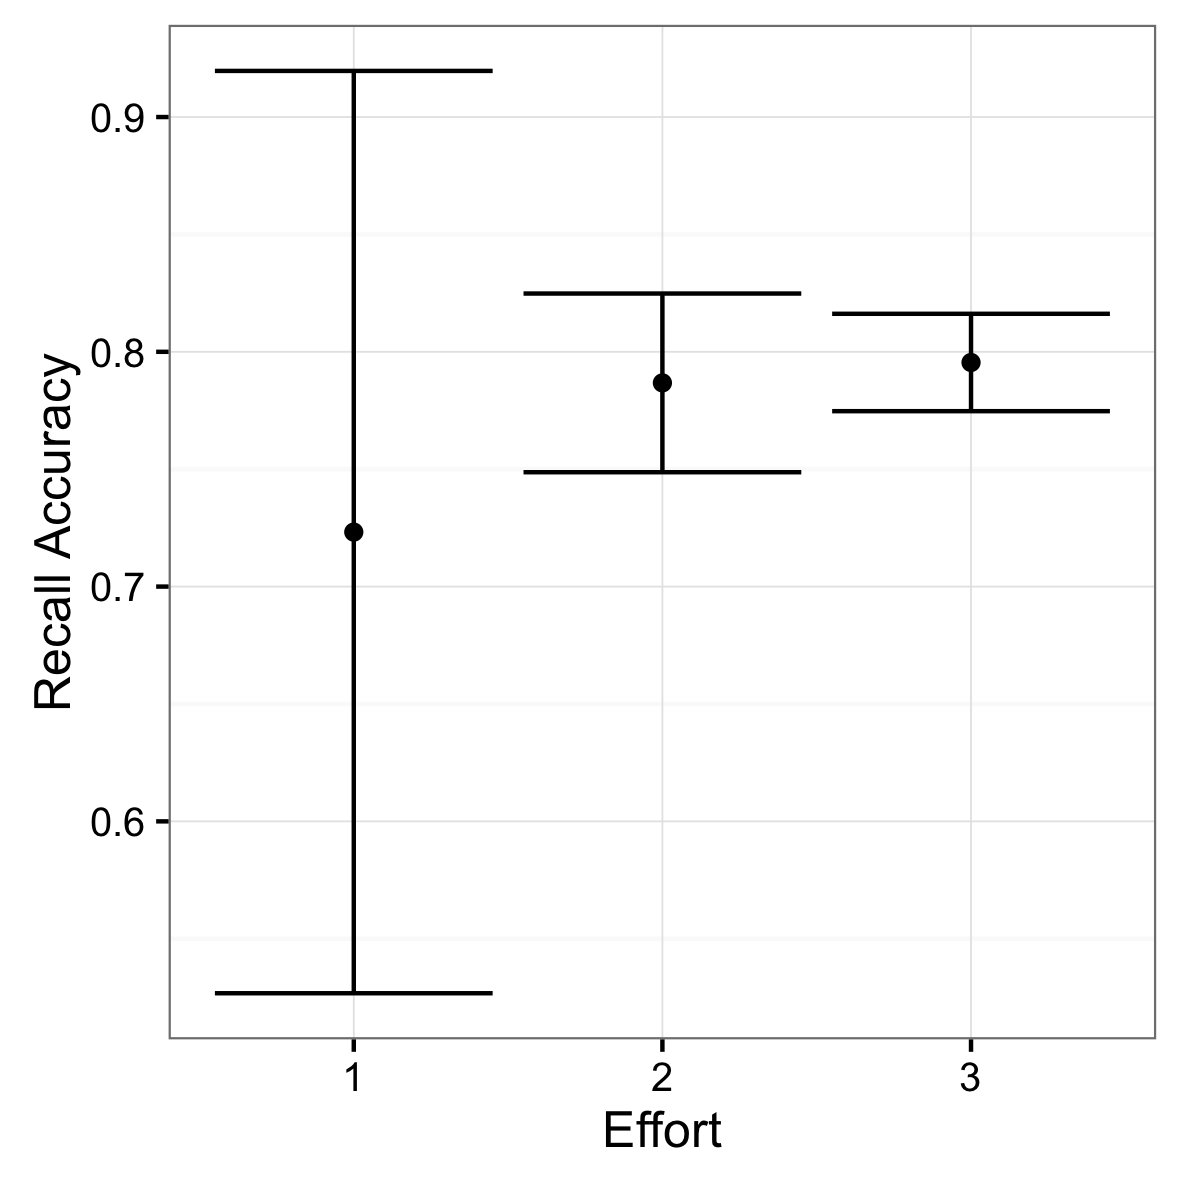
\includegraphics[width=.9\linewidth]{figures/genper_effortXoverall.png}
\caption{Self reported task effort on a 4-item Lickert scale (zeros removed) with mean and standard errors of recall accuracies per subject.}
\label{fig:genper_effortXoverall}
\end{minipage}
\begin{minipage}[t]{.5\textwidth}
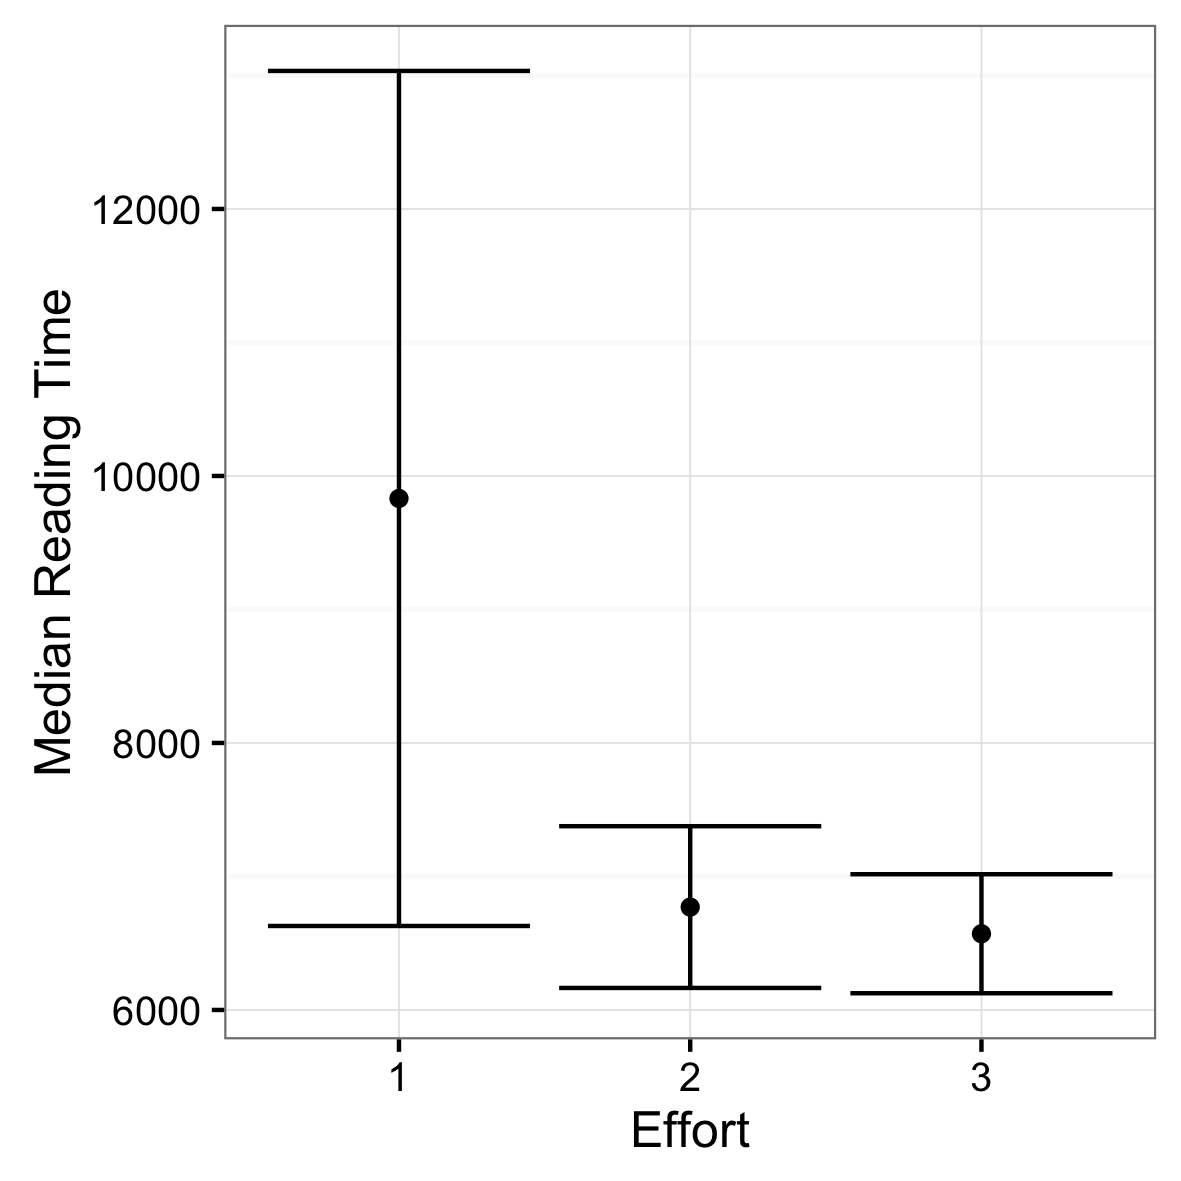
\includegraphics[width=.9\linewidth]{figures/genper_effortXtime.png}
\caption{Self reported task effort (see Fig. \ref{fig:genper_effortXoverall}) with mean and standard errors of per subject median reading time.}
\label{fig:genper_effortXtime}
\end{minipage}
\end{figure}


All in all those observations lead to the conclusion, that the task didn't reproduce a very natural reading and text comprehension environment. Participants did take a lot of time to encode or rehearse the items and I can not exclude the possibility, that participants cheated by taking notes for example.

\subsubsection{Confounding Effects}
Nonetheless I could reproduce a set of well known effects from cognition literature with this setup, which legitimizes the interpretation of our results to a certain extent.

At first, I observed a general training effect as shown in figure \ref{fig:conf_stoidx}. A univariate logistic regression predicting recall success with the trial index is highly significant (\textit{e} = 0.043, \textit{z}(9518) = 7.321,  \textit{p} < 0.001). The trials 1 and 12 seem to deviate quite strongly from the general trend. It could be the case, that even though I presented participants with a pilot statement to give them the option to get accustomed to the response menu beforehand, participants didn't fully understand the task until they completed the first trial. Further it should be noted that the trick story was inserted as the 11th trial, but of course excluded from this analysis. Apparently the lack of coherence regarding story length confused participants remarkably and is observable in recall success.

\begin{figure}
\begin{minipage}[t]{.5\textwidth}
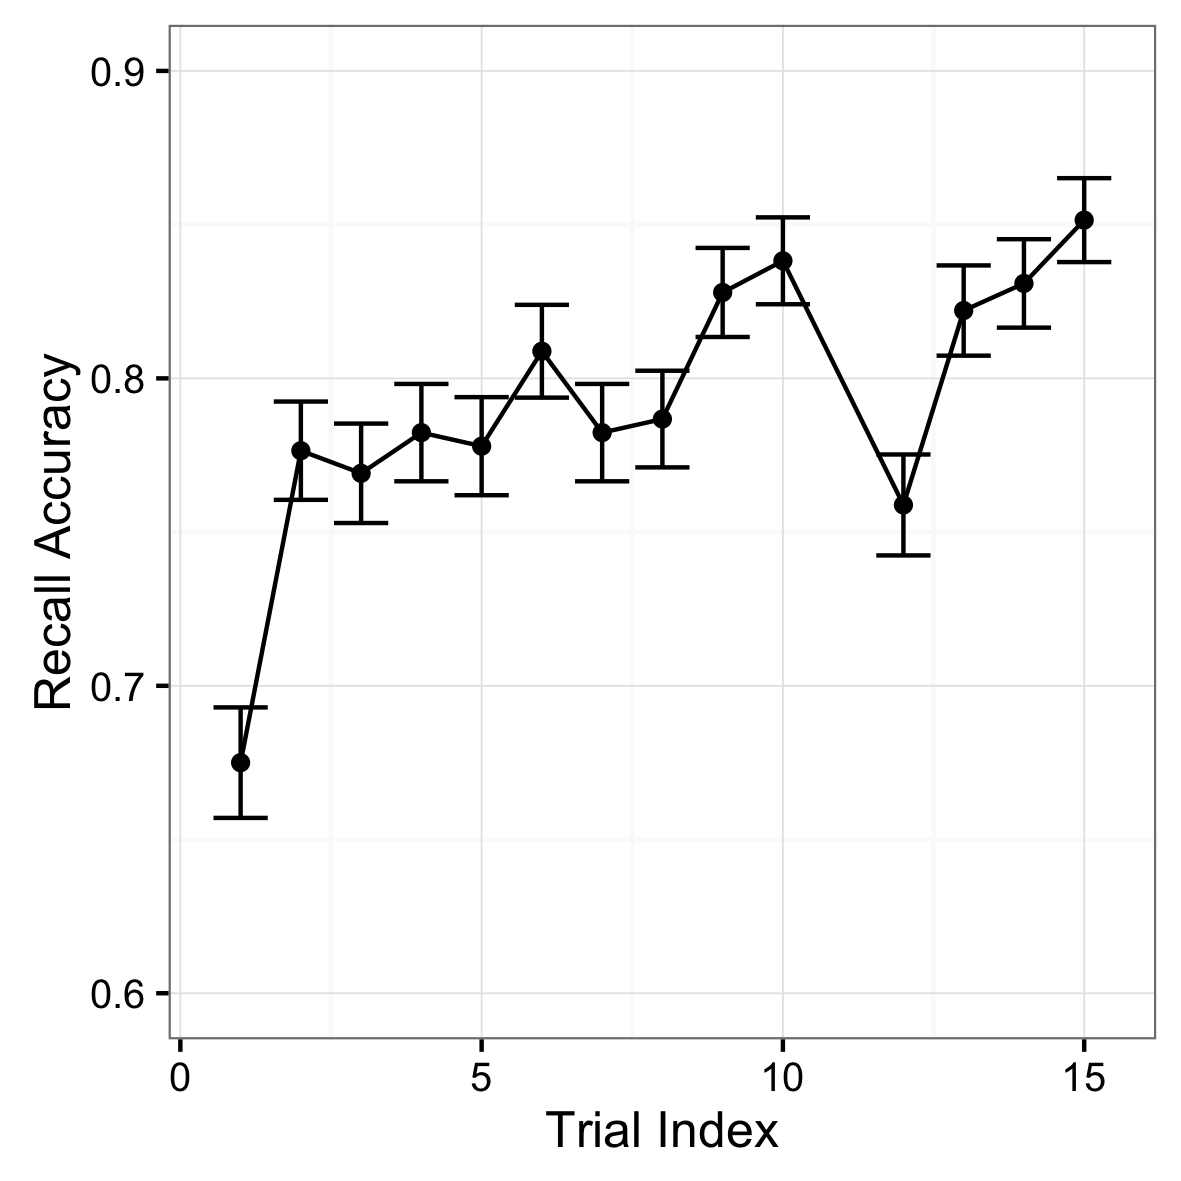
\includegraphics[width=.9\linewidth]{figures/conf_stoidx.png}
\caption{Mean recall accuracy and standard errors for each trial index.}
\label{fig:conf_stoidx}
\end{minipage}
\begin{minipage}[t]{.5\textwidth}
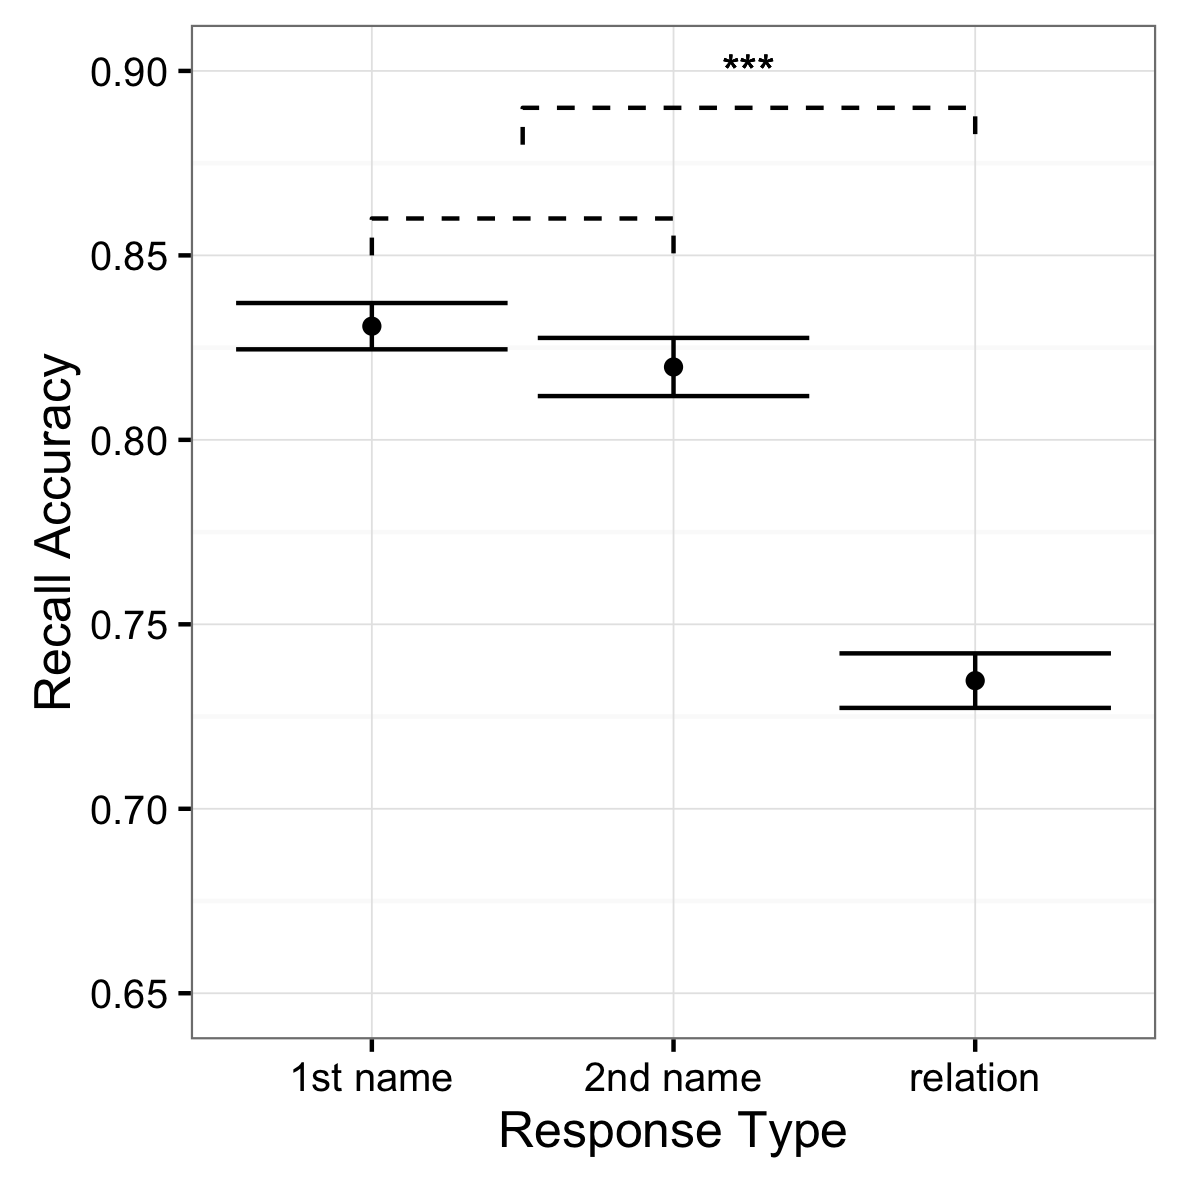
\includegraphics[width=.9\linewidth]{figures/conf_respType.png}
\caption{Mean recall accuracy and standard errors for each reponse type.}
\label{fig:conf_respType}
\end{minipage}
\end{figure}

Each statement had both entity names and relations and the first two statements had two different name responses (e.g. "Hacker Uhuy (name1) wrote (relation) computer code Wehif (name2)."). Figure \ref{fig:conf_respType} depicts the difference in recall performance for each type of response item. The two different name responses did not differ significantly (\textit{${\chi}^2$}(1, \textit{N} = 5950) = 1.219, \textit{p} = 0.270 ), therefore I grouped both name responses together for further analyses. Relation items were significantly easier to recall than entity names (\textit{${\chi}^2$}(1, \textit{N} = 9520) = 113.78, \textit{p} < 0.001 ). This effect can most probably attributed to the nonsensicality of the names, which makes them harder to recall, but it can also be argued that participants had to recall 5 names but only 3 relations. Maybe storage resources weren't equally distributed, but I will not go further into this topic.

I already analyzed the influence of median reading times per subject and detected its effect on a subjects overall recall accuracy (see General Task Performance). Therefore it is not surprising to see the same effect on the item level. The regression coefficient from the logarithm of the statement's reading time is highly significant predicting recall success in simple logistic regression (\textit{e} = 0.519, \textit{z}(9518) = 18.88, p < 0.001).

\begin{figure}
\begin{minipage}[t]{.5\textwidth}
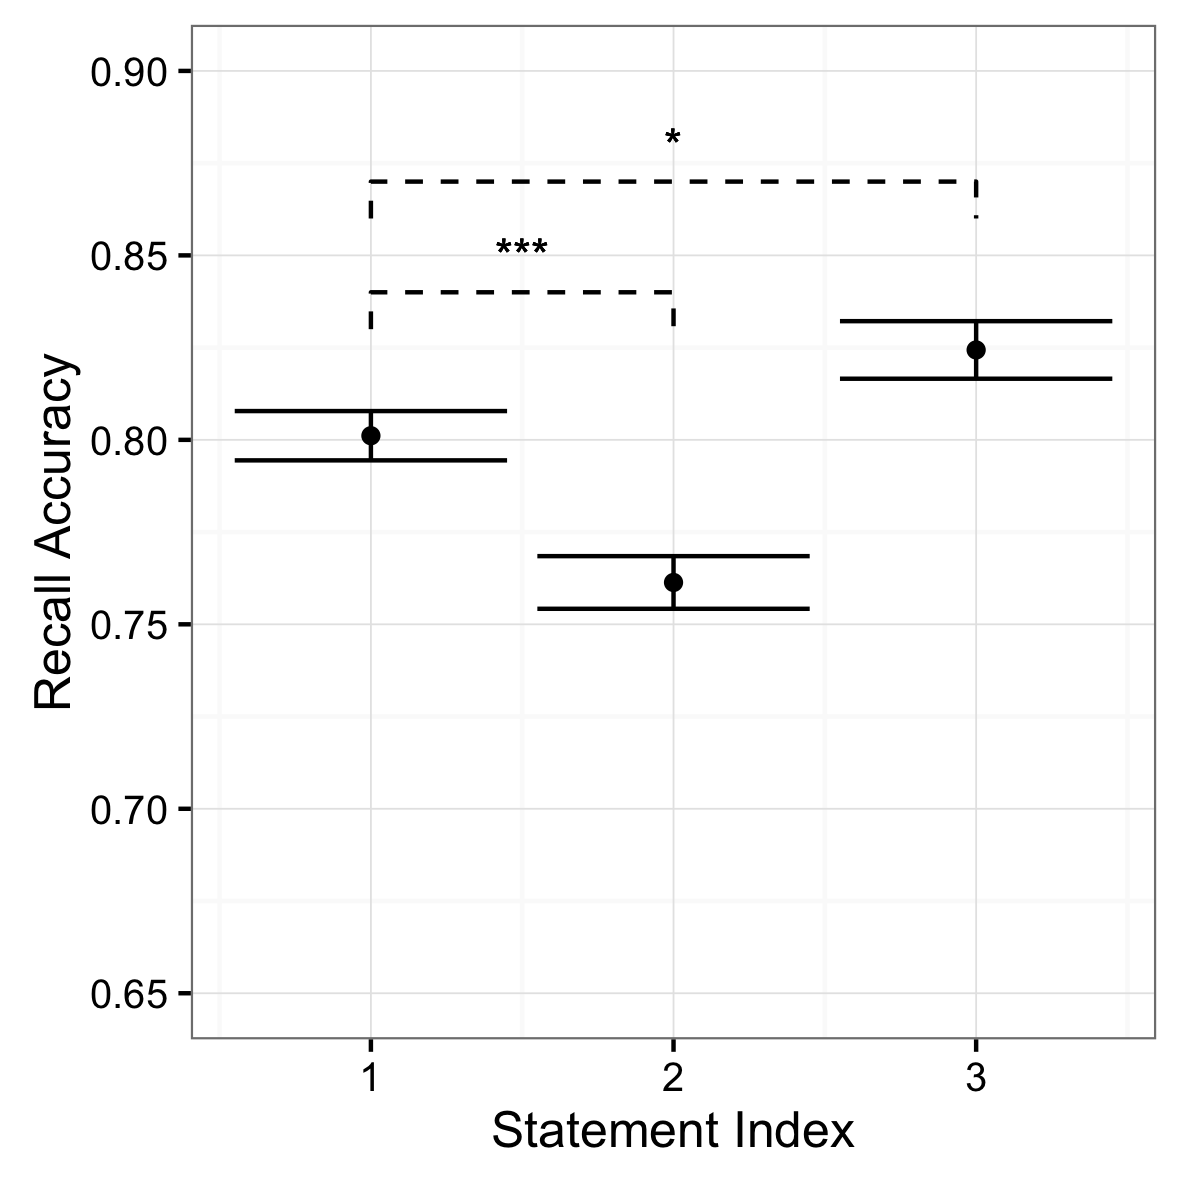
\includegraphics[width=.9\linewidth]{figures/conf_statIdx.png}
\caption{Mean recall accuracy and standard errors for each statement position.}
\label{fig:conf_statIdx}
\end{minipage}
\begin{minipage}[t]{.5\textwidth}
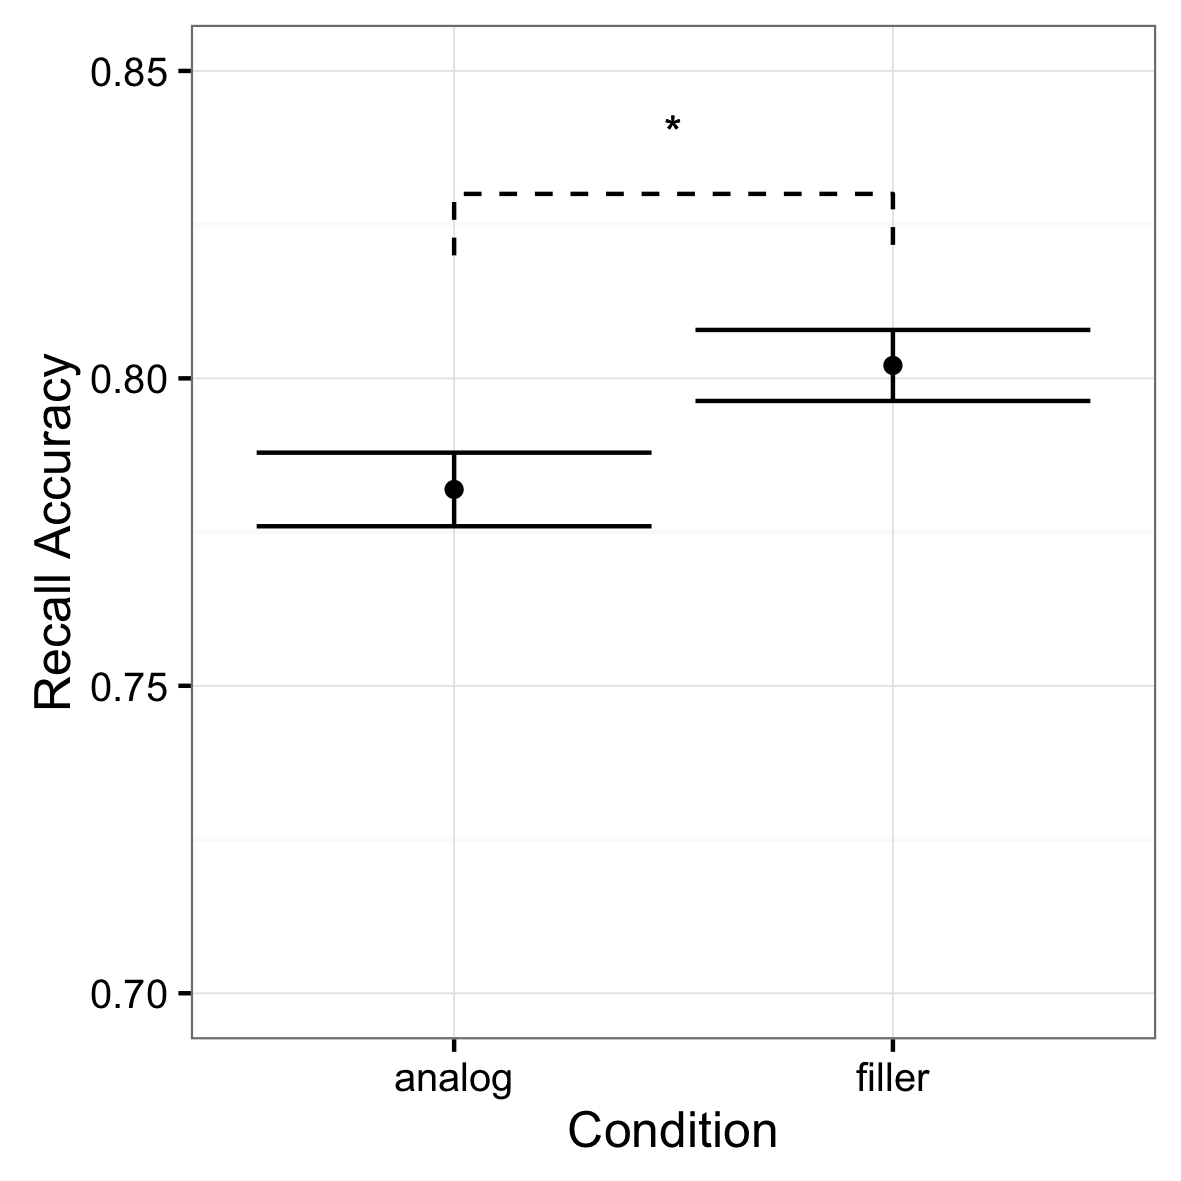
\includegraphics[width=.9\linewidth]{figures/conf_condition.png}
\caption{Mean recall accuracy and standard errors for each story structure condition.}
\label{fig:conf_condition}
\end{minipage}
\end{figure}

Because each story had three statements, I was interested, if I can replicate a primacy and recency effect. Figure \ref{fig:conf_statIdx} shows a clear difference in recall accuracy depending on the statements position in the story. A logistic regression predicting recall success with two dummy variables confirmed the statistical significance for the comparison second statement vs. first statement (\textit{e} = -0.233, \textit{z}(9517) = -4.06, \textit{p} < 0.001), and the comparison 3rd statement vs. 1st statement (\textit{e} = 0.153, (\textit{z}(9617) = 2.24, \textit{p} = 0.025). Although it should be noted, the second statement was linguistically the most complex, and the last statement in each story only had two items to remember. So it is not clear if the significant differences can be attributed to primacy/recency or rather to differing statement difficulties.

The two pools of stories, analogical and fillers, only differed very slightly in terms of recall difficulty (see figure \ref{fig:conf_condition}). The mean of recall success only differs 2\% between the conditions. Nonetheless, due to the high statistical power the dummy variable comparing analogical to filler items shows significance when analyzed with ${\chi}^2$-test (\textit{${\chi}^2$}(1, \textit{N} = 9520) = 5.877, \textit{p} = 0.015).

\subsubsection{Main Effect}
Our main hypothesis was that repeated causal structure will lead to increased memory performance. Figure \ref{fig:main} depicts the interaction of story structure condition and trial index. At first sight, it looks quite messy and not like a consistent trend. But one has to consider, that in this visualization there's still a lot of noise embedded in the form of confounding effects. I tested the interaction on statistical significance with a crossed random effects logistic regression analysis predicting recall success by adapting a method from \cite{Baayen2008}. Table \ref{table:main} shows an overview of the models tested with different confounding parameters. All models therein have a random intercept for each subject and each statement, accounting for random biases introduced by individuals and linguistic differences.

\begin{figure}
\centering
\begin{minipage}[t]{.5\textwidth}
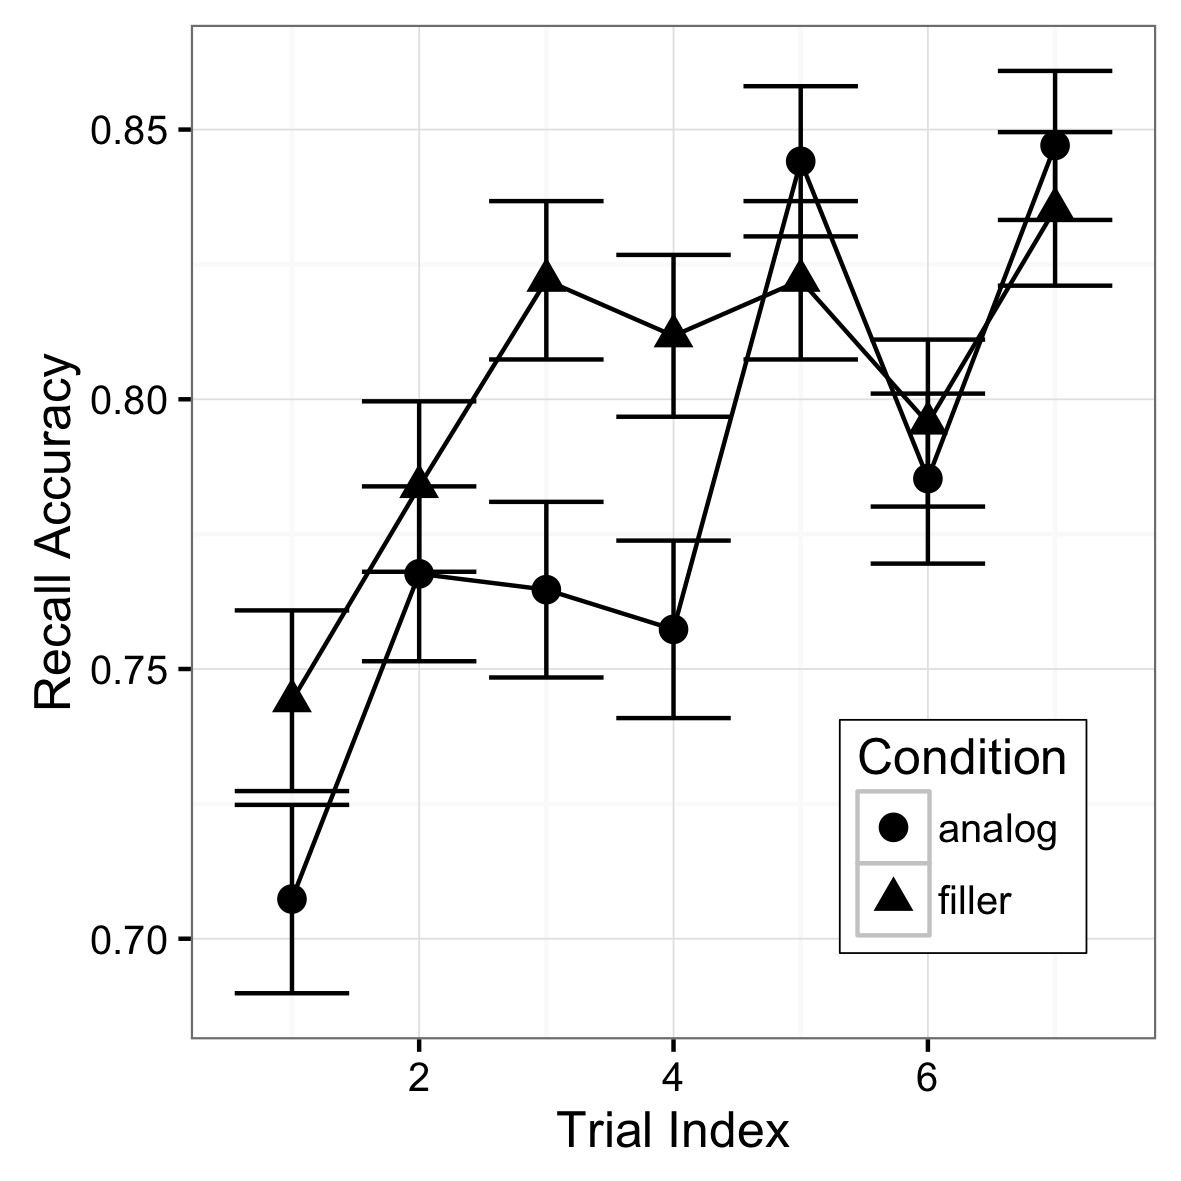
\includegraphics[width=.9\linewidth]{figures/main.png}
\caption{Mean recall accuracy and standard errors for each story position and story structure condition.}
\label{fig:main}
\end{minipage}
\end{figure}

All models from table \ref{table:main} are nested, which makes their log-likelihood comparable. The significance stars next to the log-likelihood indicates the significance level of the ${\chi}^2$-test comparing the respective model to the next simpler (the one to the left). To test the interaction, I z-transformed the variables trial index and condition (story structure: analogical vs. filler).

Model 1 is the simplest, only accounting for the single effects plus their interaction, which is our main focus. Bear in mind that those models are crossed random effects models with random subject and statement intercepts. I can see that trial index has a strong effect on recall success, which has already been visible in the figures \ref{fig:main} and \ref{fig:conf_stoidx}. The interaction seems to be not too far off from significance but has not reached the 5\%-cutoff. Although when adding additional controlling parameters (as in model 2, 3 and 4), the main interaction become more and more significant mainly due to its increased estimate. As suspected, the fit of the models increases when controlling for the confounding effects. According to the ${\chi}^2$-tests the loss of degrees of freedom seem justified. it is noteworthy that the increase in fit is quite large when adding the log of the reading reading (model 4), compared to the increase in fit when adding "Statement Nr" (model 3).

\begin{landscape}

% Table created by stargazer v.5.2 by Marek Hlavac, Harvard University. E-mail: hlavac at fas.harvard.edu
% Date and time: Thu, Aug 11, 2016 - 00:30:34
\begin{table}
\centering
  \caption{}
  \label{table:main}
\small
\renewcommand{\arraystretch}{0.45}
\begin{tabular}{@{\extracolsep{5pt}}lcccccc}
\\[-1.8ex]\hline
\hline \\[-1.8ex]
 & \multicolumn{6}{c}{\textit{Dependent variable:}} \\
\cline{2-7}
\\[-1.8ex] & \multicolumn{6}{c}{Recall Sucess} \\
\\[-1.8ex] & (1) & (2) & (3) & (4) & (5) & (6)\\
\hline \\[-1.8ex]
 Trial Index & 0.218$^{**}$ & 0.223$^{**}$ & 0.222$^{**}$ & 0.280$^{**}$ & 0.327$^{**}$ & 0.256$^{**}$ \\
  & (0.028) & (0.028) & (0.028) & (0.029) & (0.031) & (0.034) \\
  & & & & & & \\
 Condition & 0.071 & 0.073 & 0.072$^{*}$ & 0.076$^{*}$ & 0.071$^{o}$ & 0.069$^{o}$ \\
  & (0.045) & (0.051) & (0.036) & (0.038) & (0.038) & (0.037) \\
  & & & & & & \\
 Response Type Relation &  & $-$0.703$^{**}$ & $-$0.724$^{**}$ & $-$0.738$^{**}$ & $-$0.740$^{**}$ & $-$0.743$^{**}$ \\
  &  & (0.057) & (0.057) & (0.058) & (0.058) & (0.058) \\
  & & & & & & \\
 Statement Nr 2 &  &  & $-$0.289$^{**}$ & $-$0.022 & $-$0.023 & $-$0.023 \\
  &  &  & (0.083) & (0.092) & (0.090) & (0.088) \\
  & & & & & & \\
 Statement Nr 3 &  &  & 0.311$^{**}$ & 0.938$^{**}$ & 0.941$^{**}$ & 0.943$^{**}$ \\
  &  &  & (0.093) & (0.113) & (0.112) & (0.110) \\
  & & & & & & \\
 Log Reading Time &  &  &  & 0.542$^{**}$ & 0.544$^{**}$ & 0.545$^{**}$ \\
  &  &  &  & (0.048) & (0.048) & (0.048) \\
  & & & & & & \\
 After Trick &  &  &  &  & $-$0.566$^{**}$ & $-$0.535$^{**}$ \\
  &  &  &  &  & (0.112) & (0.112) \\
  & & & & & & \\
 First &  &  &  &  &  & $-$0.547$^{**}$ \\
  &  &  &  &  &  & (0.110) \\
  & & & & & & \\
 Trial Index:Condition & $-$0.052$^{o}$ & $-$0.053$^{o}$ & $-$0.055$^{o}$ & $-$0.057$^{*}$ & $-$0.063$^{*}$ & $-$0.057$^{*}$ \\
  & (0.028) & (0.028) & (0.028) & (0.029) & (0.029) & (0.028) \\
  & & & & & & \\
 Constant & 1.726$^{**}$ & 2.036$^{**}$ & 2.051$^{**}$ & $-$2.838$^{**}$ & $-$2.810$^{**}$ & $-$2.780$^{**}$ \\
  & (0.139) & (0.146) & (0.149) & (0.449) & (0.449) & (0.449) \\
  & & & & & & \\
\hline \\[-1.8ex]
Observations & 9,520 & 9,520 & 9,520 & 9,520 & 9,520 & 9,520 \\
Log Likelihood & $-$4,191.375 & $-$4,116.757$^{***}$ & $-$4,101.298$^{***}$ & $-$4,030.975$^{***}$ & $-$4,018.804$^{***}$ & $-$4,006.802$^{***}$ \\
Akaike Inf. Crit. & 8,394.750 & 8,247.515 & 8,220.596 & 8,081.950 & 8,059.609 & 8,037.605 \\
Bayesian Inf. Crit. & 8,437.717 & 8,297.643 & 8,285.046 & 8,153.562 & 8,138.381 & 8,123.538 \\
\hline
\hline \\[-1.8ex]
\textit{Note:}  & \multicolumn{6}{r}{	\textsuperscript{o} p<0.1; * p<0.05; ** p<0.01; *** p<0.001} \\
\end{tabular}
\end{table}

\end{landscape}

To account for two anomalies in our data, I tested two additional models adding a free trial position parameter on each, the first parameter being "after trick". As I have seen in figure \ref{fig:conf_stoidx}, recall success remarkably declines after the insertion of the trick story in our trial sequence. To investigate the effect of this incoherence on our main interaction, I ran the logistic regression in model 5 with an extra free parameter for all trials after the trick story. Not surprisingly the log-likelihood of this model increases significantly, and the coefficient estimate for interaction is bigger then in the previous models.

The other anomaly from inspecting the effect of trial index on recall accuracy (fig. \ref{fig:conf_stoidx}) was the big deviation at the first trial. To investigate if the statistical power of the interaction mainly results from this deviation, I embedded another free parameter for all first trials. In model 6 a slightly decreased coefficient estimate in the interaction in model 6 can be observed, which stays below the 5\%-significance level.

\begin{figure}
\centering
\begin{minipage}[t]{.5\textwidth}
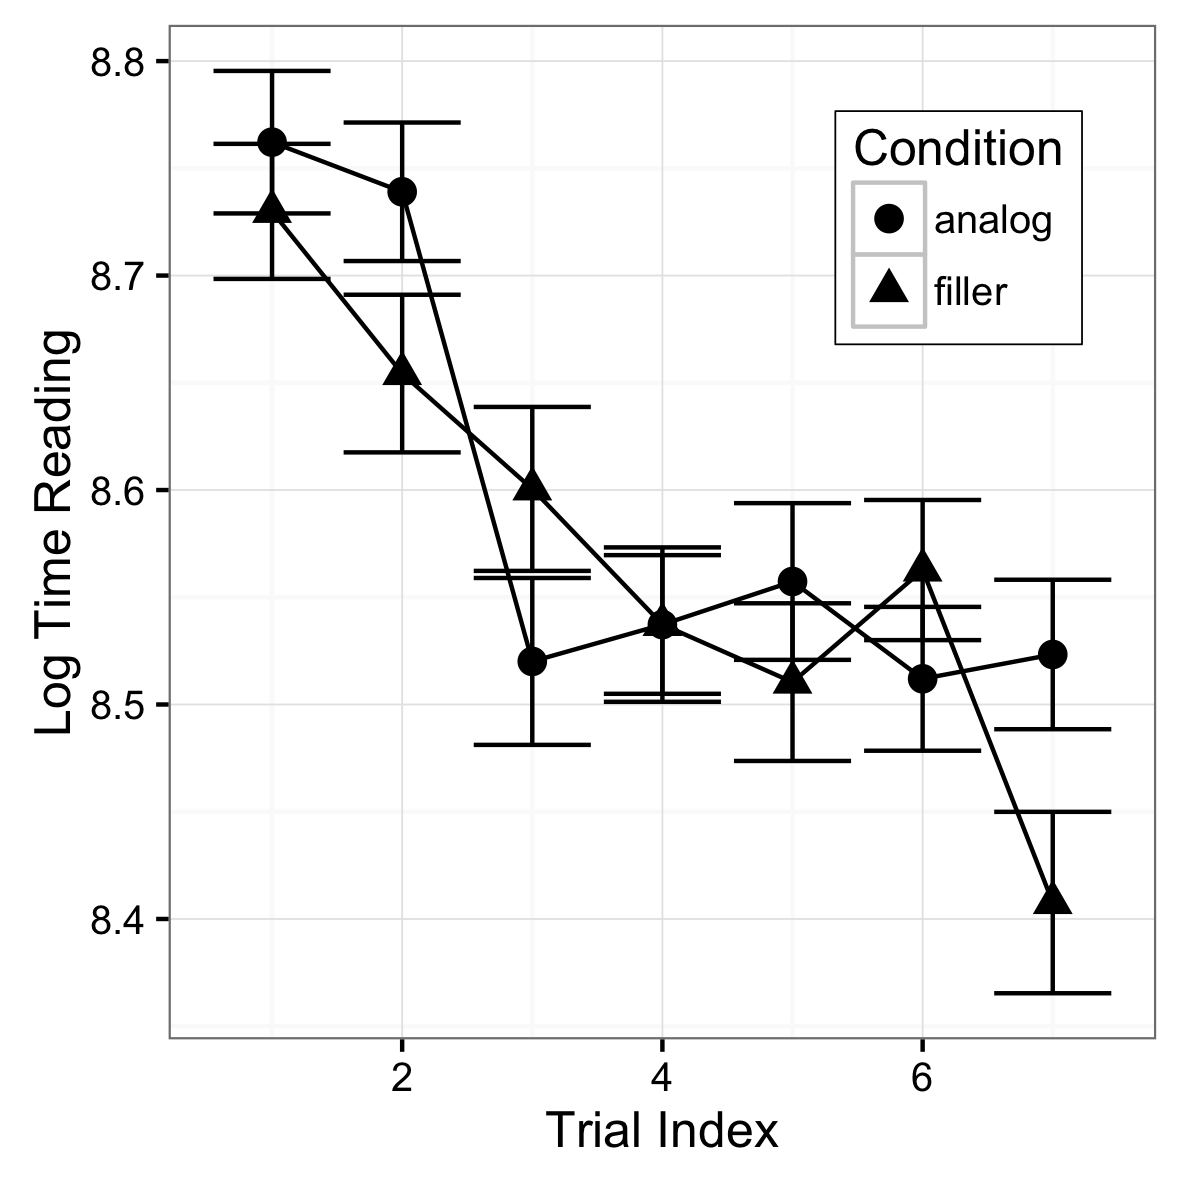
\includegraphics[width=.9\linewidth]{figures/read.png}
\caption{Mean and standard errors of the logarithm of the reading time in milliseconds for each trial index and story structure condition.}
\label{fig:read}
\end{minipage}
\end{figure}

\cite{Day2007} observed decreased encoding time when participants read a story which was structurally similar to the previous story. Therefore I also tested the effect of repeated causal structure on encoding time with a crossed random effects regression analysis, similar to when predicting recall success. This time it is not a logistic but a linear model. Also, the linear regression runs on the level of the statement (N=3570), and not item (N=9520). The interaction of story structure structure with trial index does not reach significance (see table \ref{table:read}). It is important to mention that our task crucially differed from \cite{Day2007} in the sense, that I specifically ask our participants to remember the different pieces of a very short story, while \cite{Day2007} have asked the participants to actually comprehend a story with the expectation to answer questions about it. Also our material differs a lot from the material of \cite{Day2007} in terms of complexity and conventionality.


% Table created by stargazer v.5.2 by Marek Hlavac, Harvard University. E-mail: hlavac at fas.harvard.edu
% Date and time: Thu, Aug 11, 2016 - 10:22:48
\begin{table} \centering
  \small
  \caption{Regression Coefficient and Standard Errors in Parentheses from Experiment 1}
  \label{table:read}
  \renewcommand{\arraystretch}{0.6}
\begin{tabular}{@{\extracolsep{5pt}}lcc}
\\[-1.8ex]\hline
\hline \\[-1.8ex]
 & \multicolumn{2}{c}{\textit{Linear Regression Models predicting the Logarithm of Time Reading:}} \\
\cline{2-3}
\\[-1.8ex] & (1) & (2)\\
\hline \\[-1.8ex]
 Trial Index & $-$0.082$^{**}$ & $-$0.082$^{**}$ \\
  & (0.010) & (0.010) \\
  & & \\
 Condition & $-$0.007 & $-$0.007 \\
  & (0.070) & (0.013) \\
  & & \\
 Statement Nr 2 &  & $-$0.422$^{**}$ \\
  &  & (0.032) \\
  & & \\
 Statement Nr 3 &  & $-$1.064$^{**}$ \\
  &  & (0.032) \\
  & & \\
 Trial Index:Condition & $-$0.004 & $-$0.004 \\
  & (0.010) & (0.010) \\
  & & \\
 Constant & 8.511$^{**}$ & 9.007$^{**}$ \\
  & (0.094) & (0.067) \\
  & & \\
\hline \\[-1.8ex]
Observations & 3,570 & 3,570 \\
Log Likelihood & $-$3,485.351 & $-$3,421.937$^{***}$ \\
Akaike Inf. Crit. & 6,984.703 & 6,861.874 \\
Bayesian Inf. Crit. & 7,027.965 & 6,917.497 \\
\hline
\hline \\[-1.8ex]
\textit{Note:}  & \multicolumn{2}{r}{	\textsuperscript{o} p<0.1; * p<0.05; ** p<0.01; *** p<0.001} \\
\end{tabular}
\end{table}


\subsubsection{Post-Experiment Questionnaire}

\begin{figure}
\begin{minipage}[t]{.5\textwidth}
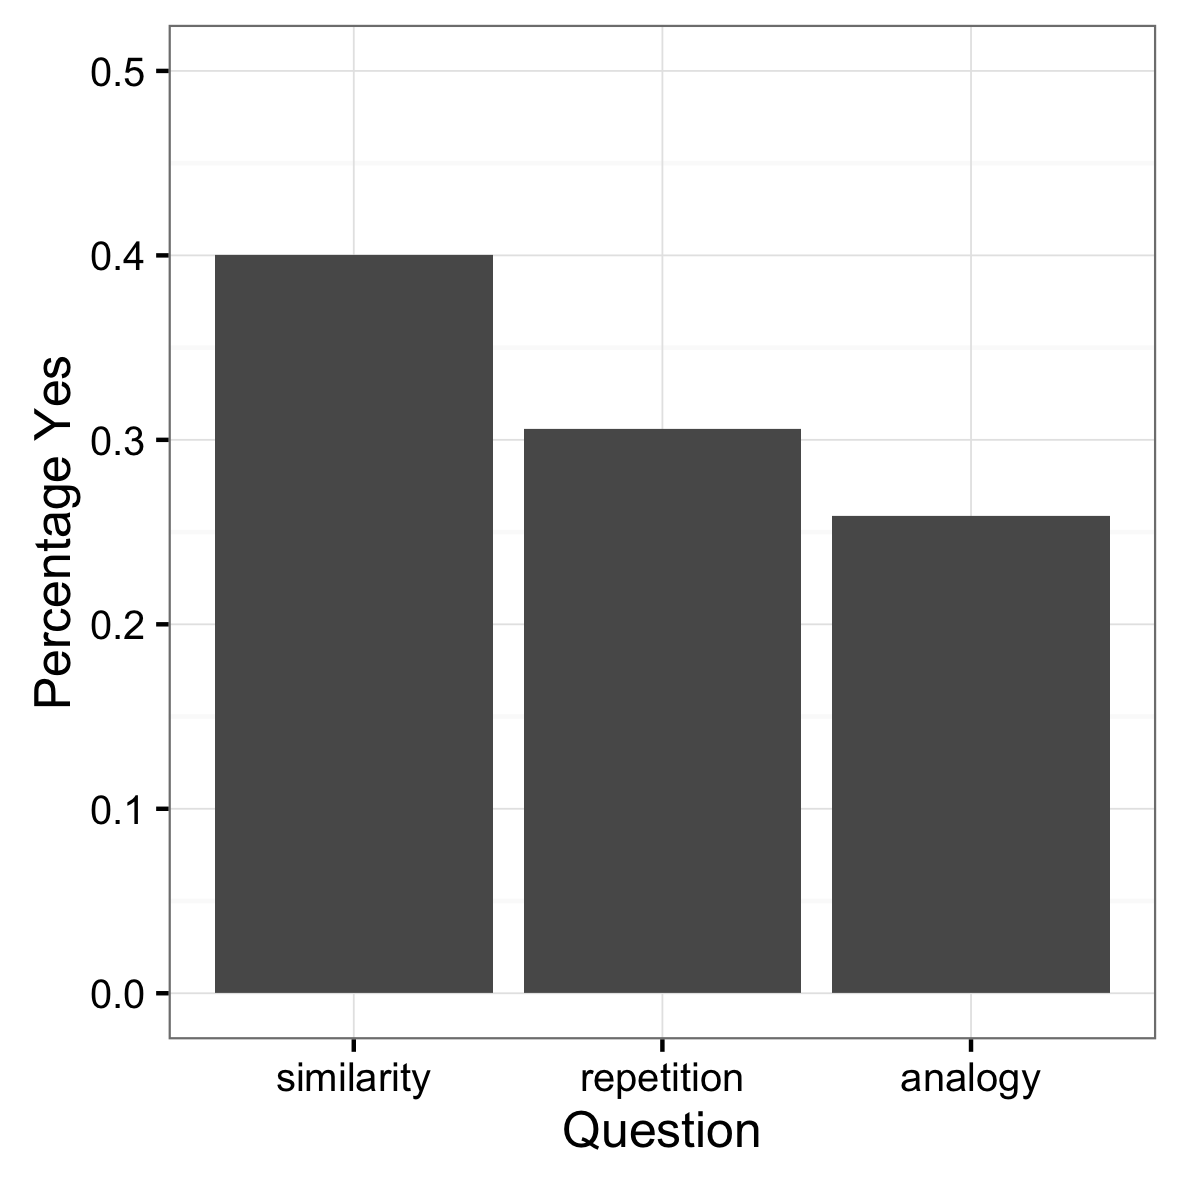
\includegraphics[width=.9\linewidth]{figures/fol_percYes.png}
\caption{Percentage of positive responses to the three follow-up questions.}
\label{fig:fol_percYes}
\end{minipage}
\begin{minipage}[t]{.5\textwidth}
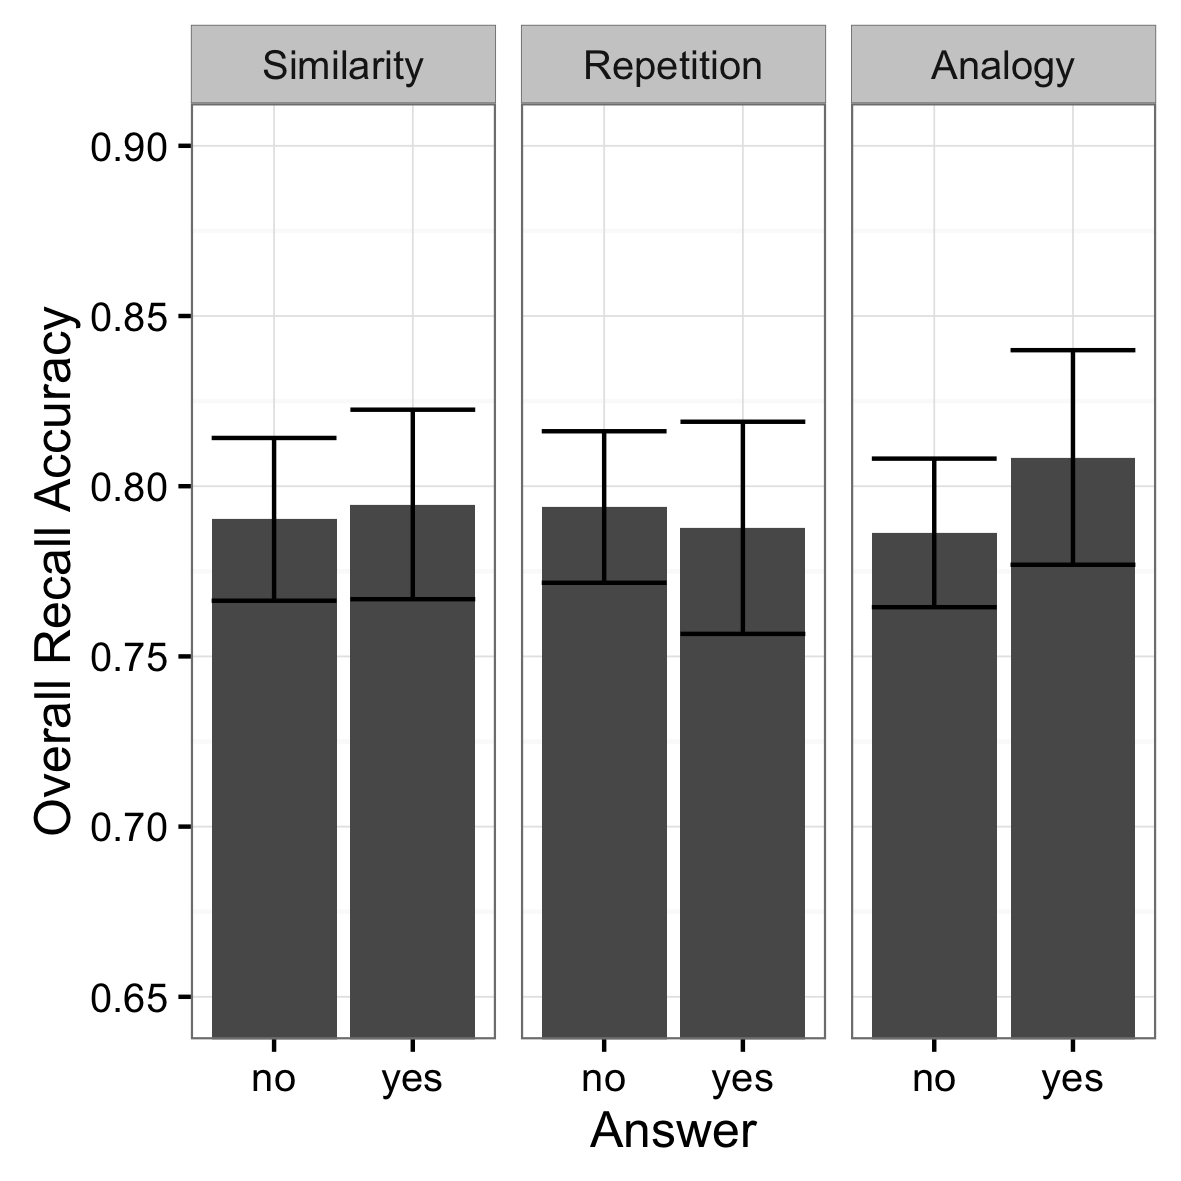
\includegraphics[width=.9\linewidth]{figures/fol_answerXoverall.png}
\caption{Mean and standard error of subjects overall recall accuracy for each response to the three follow-up questions.}
\label{fig:fol_answerXoverall}
\end{minipage}
\end{figure}

I claim that any analogical transfer in this experiment is unintentional, because participants are supposed to recall content and aren't told to explicitly compare stories to each other or even are aware of the systematicity. To check to what extent participants were aware of the repeated analogical structure I asked three post-experiment questions. The percentages of our sample that detected certain kinds of similarities between the stories are shown in figure \ref{fig:fol_percYes}. While 40\% reported to notice similarities between the stories, when asked to explain their response, most participants mentioned that all stories had nonsensical names. Some also mentioned the linguistic coherence ("Every story had 3 names of places, things or people.", "Every story had 2 actions and 1 consequence"). 31\% reported to having noticed repeating elements. The open answers were quite similar to the previous question. Only 26\% of our sample said to having noticed the repeating analog/causal structure in every second story. Their open responses reveal, that often they meant the syntactic similarity instead of the causal structure. Only a 4 participants really detected the repeating analogical structure, indicating that the big majority of people could not have intentionally mapped stories on to each other.

I further investigated if detection of certain kinds of similarities between the stories had an effect on subject's overall recall accuracy. Figure \ref{fig:fol_answerXoverall} depicts those comparisons, which seem to not make a difference. Running simple linear regressions also showed no significant effect for any of the questions (see Table \ref{table:fol}), indicating that being aware of any kind of shared similarity did not yield any benefit in memory performance.


% Table created by stargazer v.5.2 by Marek Hlavac, Harvard University. E-mail: hlavac at fas.harvard.edu
% Date and time: Fri, Aug 12, 2016 - 20:54:33
\begin{table}[!htbp] \centering
  \caption{}
  \label{table:fol}
  \small
  \renewcommand{\arraystretch}{0.6}
\begin{tabular}{@{\extracolsep{5pt}}lccc}
\\[-1.8ex]\hline
\hline \\[-1.8ex]
 & \multicolumn{3}{c}{\textit{Dependent variable:}} \\
\cline{2-4}
\\[-1.8ex] & \multicolumn{3}{c}{Overall Recall Accuracy} \\
\\[-1.8ex] & (1) & (2) & (3)\\
\hline \\[-1.8ex]
 Similarity & 0.004 &  &  \\
  & (0.037) &  &  \\
  & & & \\
 Repetition &  & $-$0.006 &  \\
  &  & (0.039) &  \\
  & & & \\
 Analogy &  &  & 0.022 \\
  &  &  & (0.041) \\
  & & & \\
 Constant & 0.790$^{**}$ & 0.794$^{**}$ & 0.786$^{**}$ \\
  & (0.023) & (0.022) & (0.021) \\
  & & & \\
\hline \\[-1.8ex]
Observations & 85 & 85 & 85 \\
R$^{2}$ & 0.0002 & 0.0003 & 0.003 \\
Adjusted R$^{2}$ & $-$0.012 & $-$0.012 & $-$0.009 \\
Residual Std. Error (df = 83) & 0.167 & 0.167 & 0.167 \\
F Statistic (df = 1; 83) & 0.014 & 0.024 & 0.287 \\
\hline
\hline \\[-1.8ex]
\textit{Note:}  & \multicolumn{3}{r}{\textsuperscript{o} p<0.1; * p<0.05; ** p<0.01; *** p<0.001} \\
\end{tabular}
\end{table}


\subsection{Conclusion}
In this experiment I have discovered various weaknesses in the experimental setting. Nonetheless I could replicate a set of well known effects. Plus, there seems to be weak evidence for an increased learning rate with repeated causal structure. To strengthen our argument for analogical transfer in this Hebb repetition paradigm, I decided to conduct another experiment, hoping to improve the methods where I see them unfit.

\newpage
\section{Experiment 2}
Whereas in experiment 1 only weak evidence for increased memory performance in repeated analogical stories could be detected, it could still be the case, that the effect is overshadowed by the change of story structure after each story. This is different to relational priming studies, where the effect was usually observed when the same relation was activated just before the cued word pair. That's why I decided to investigate another experimental setting with repeated story structures.
Another surprise in experiment 1 was the overall high recall success rate. Participants were taking a lot of time to encode and/or rehearse the information, a lot more than I'd expect in a natural reading environment. I therefore decided to change the free reading time to a fixed time.
Due to the anomalies at trial position 1 and 11 in experiment 1, a third category of stories was introduced, the so called burn-in stories. These stories solely served the purpose of reducing noise from unintended trial sequence effects at the very beginning and after the trick story. They have the same characterization as the filler stories.

\subsection{Methods}
The methods were the same as in Experiment 1 with following exceptions.

\subsubsection{Participants}
I again collected observations from 78 participants on Crowdflower. Applying the same exclusions criteria as in experiment 1, I ended up with a sample of 62 participants. Median age was 28 years, which is remarkably lower than in experiment 1 (see figure \ref{fig:sample2_age}). Qualification was equally balanced between high-school and university degrees (each 50\%). 60\% percent of our sample was female.

\begin{figure}
\centering
\begin{minipage}[t]{.9\textwidth}
\small
\begin{tabular}{| l | c | c | c | c | c | c | c | c | c | c | c | c | c | c | c | c | c |}
  \multicolumn{18}{c}{ }\\
  \hline
  \multicolumn{1}{| l }{Trial Sequences} & \multicolumn{17}{c |}{ } \\ \hline
  S1: & \cellcolor{black!10}B & \cellcolor{black!10}B & \cellcolor{black!10}B & \cellcolor{black!30}A & \cellcolor{black!30}A & F & F & \cellcolor{black!30}A & \cellcolor{black!30}A & F & F & \cellcolor{black!65}T & \cellcolor{black!10}B & \cellcolor{black!30}A & \cellcolor{black!30}A & F & F \\ \hline
  S2: & \cellcolor{black!10}B & \cellcolor{black!10}B & \cellcolor{black!10}B & F & F & \cellcolor{black!30}A & \cellcolor{black!30}A & F & F & \cellcolor{black!30}A & \cellcolor{black!30}A & \cellcolor{black!65}T & \cellcolor{black!10}B & F & F & \cellcolor{black!30}A & \cellcolor{black!30}A \\ \hline
\end{tabular}
\caption{Note: A=analog, B=burn-in, F=filler, T=trick}
\label{fig:seq2}
\end{minipage}
\end{figure}

\subsubsection{Material}
To further balance story difficulties I replaced a few outlier stories with new ones. Because of the additional need of filler stories, I constructed a few new ones. To see the full list of stories used in this experiment see the appendix.

\subsubsection{Procedure}
In the preview description on CrowdFlower I changed the wording a little, because I didn't want participants to focus too much on effort. So I told them that they will get the bonus only if they pay attention to the task throughout the experiment, and that I will probe their attention. This way I also wanted to reduce the incentive to cheat. Performance should not play a role in payment.
The biggest change in experiment 2 is the introduction of a fixed reading time and a burn-in phase at the beginning and after the trick story. Also the story structure sequence changed to a pairwise repeated design.  Figure \ref{fig:seq2} offers an overview of the two possible trial sequences in this experiment. Participants were assigned randomly to one of those timelines. For each statement participants had 3 seconds to encode the information, which is less then half of the median reading time from experiment 1.

\begin{figure}
\begin{minipage}[t]{.5\textwidth}
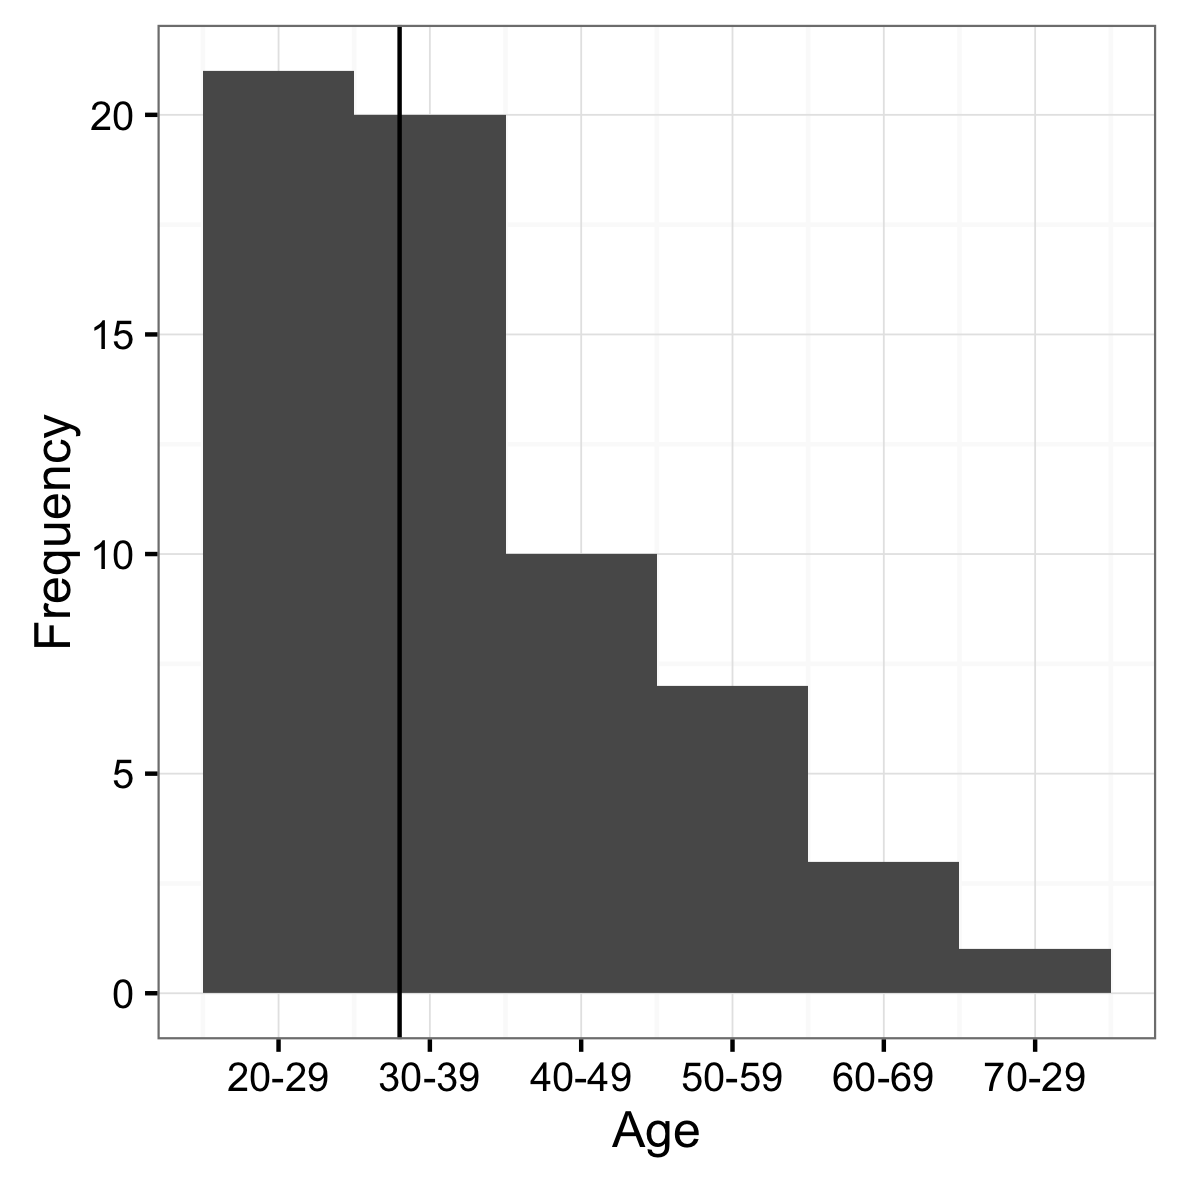
\includegraphics[width=.9\linewidth]{figures/sample2_age.png}
\caption{Distribution of age plus median in the sample of experiment 2.}
\label{fig:sample2_age}
\end{minipage}
\begin{minipage}[t]{.5\textwidth}
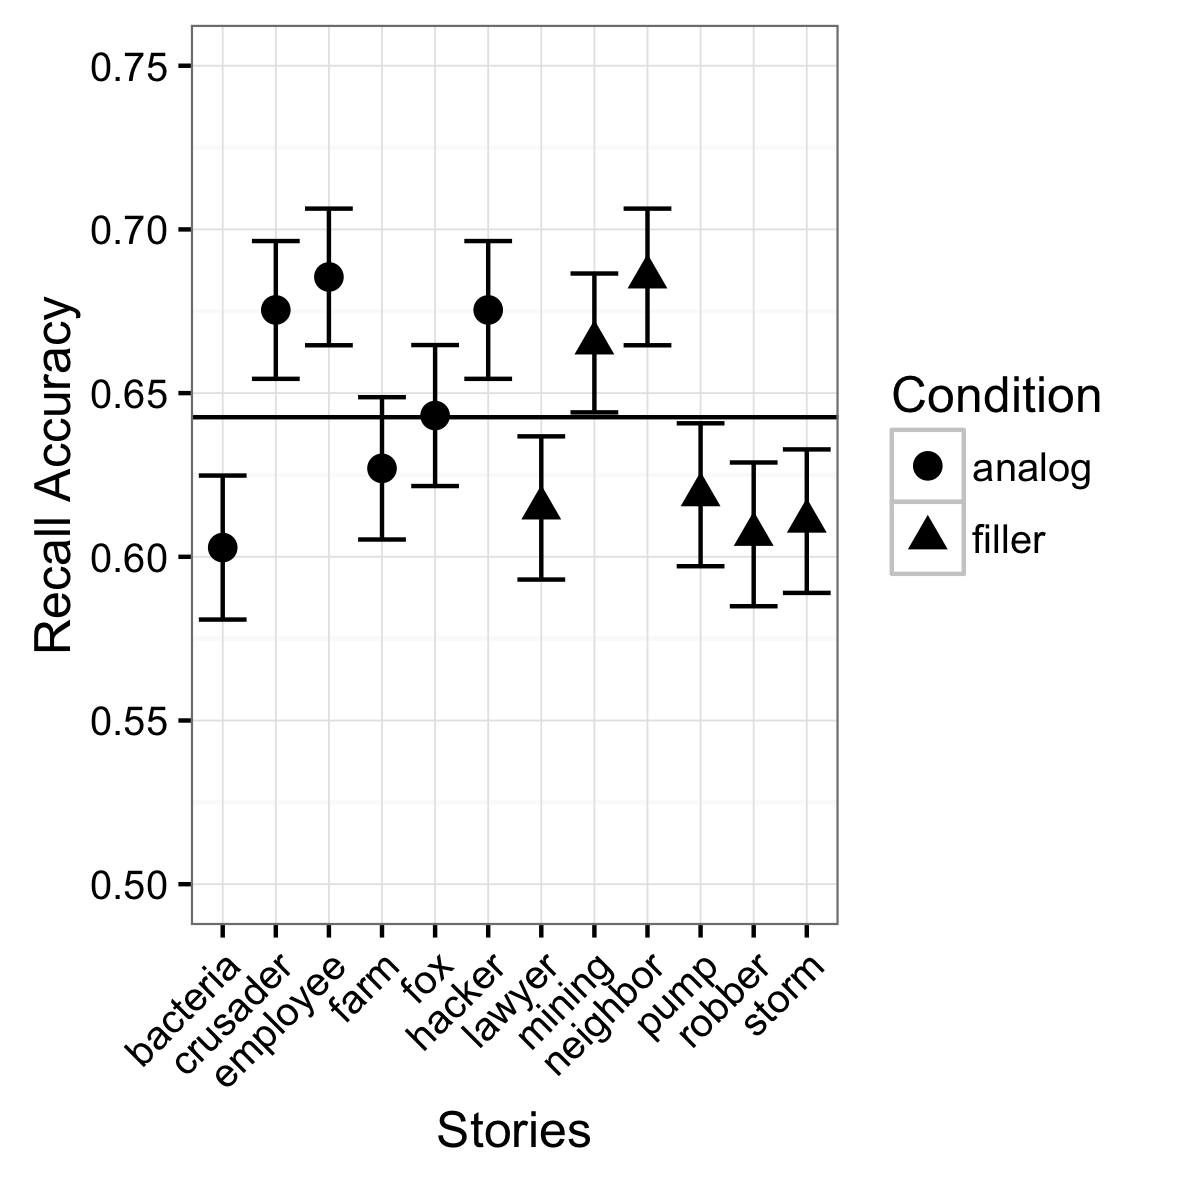
\includegraphics[width=.9\linewidth]{figures/material2_stories.png}
\caption{Mean and standard error of recall accuracy for each story with grand mean.}
\label{fig:material2_stories}
\end{minipage}
\end{figure}

\subsection{Results and Discussion}
I will only present and discuss results where they deviate from experiment 1.

\subsubsection{Material Assessment}
Even though I tried to equate the difficulties between the stories, it seems the reduced encoding time has introduced more sensitivity regarding story difficulty to the task (see figure \ref{fig:material2_stories}). The standard deviation between the stories mean recall accuracies is bigger in experiment 2 than in experiment 1. Although the Levene test for homogeneity of variances is just marginally significant (\textit{F}(1,24) = 3.082, \textit{p} = 0.091). The analysis of variance investigating overall recall accuracies for each story is again significant, but because there are less observations in experiment 2, the significance is on a lower level ( \textit{F}(11,5940) = 2.318, \textit{p} = 0.008).

\subsubsection{General Task Performance}
Setting a time limit during encoding clearly had a big impact on recall accuracy. Figure \ref{fig:genper_overall} depicts the distribution of participants' overall recall accuracy. Median is at 67\% recall accuracy, more than 10\% lower than in experiment 1. A Welch two sample t-test between subjects' overall recall accuracies from experiment 1 and 2 showed high significance (\textit{t}(147)=4.74, \textit{p} < 0.001). As a result from the increased difficulty, also the sensitivity to an individual's performance increased. The Levene test for homogeneity of variances between participants' overall accuracies of experiment 1 and 2 showed a significant result (\textit{F}(1,145) = 4.0749, \textit{p} = 0.045), meaning the variance of individual performances in experiment 2 is significantly bigger than in experiment 1.

\begin{figure}
\begin{minipage}[t]{.5\textwidth}
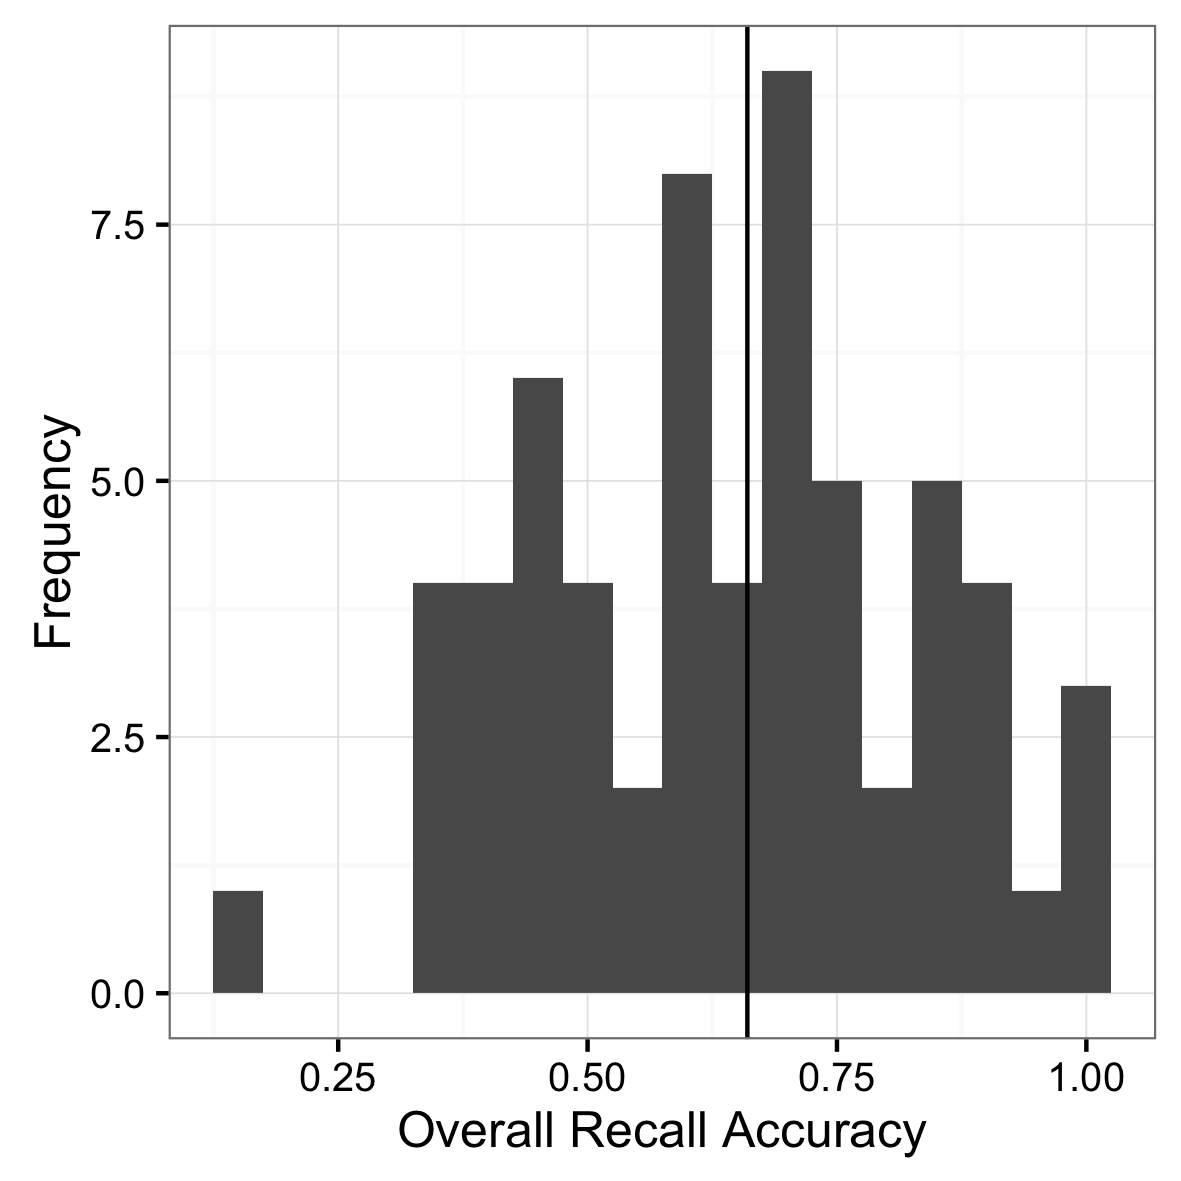
\includegraphics[width=.9\linewidth]{figures/genper2_overall.png}
\caption{Distribution of subjects' overall recall accuracy with median.}
\label{fig:genper2_overall}
\end{minipage}
\begin{minipage}[t]{.5\textwidth}
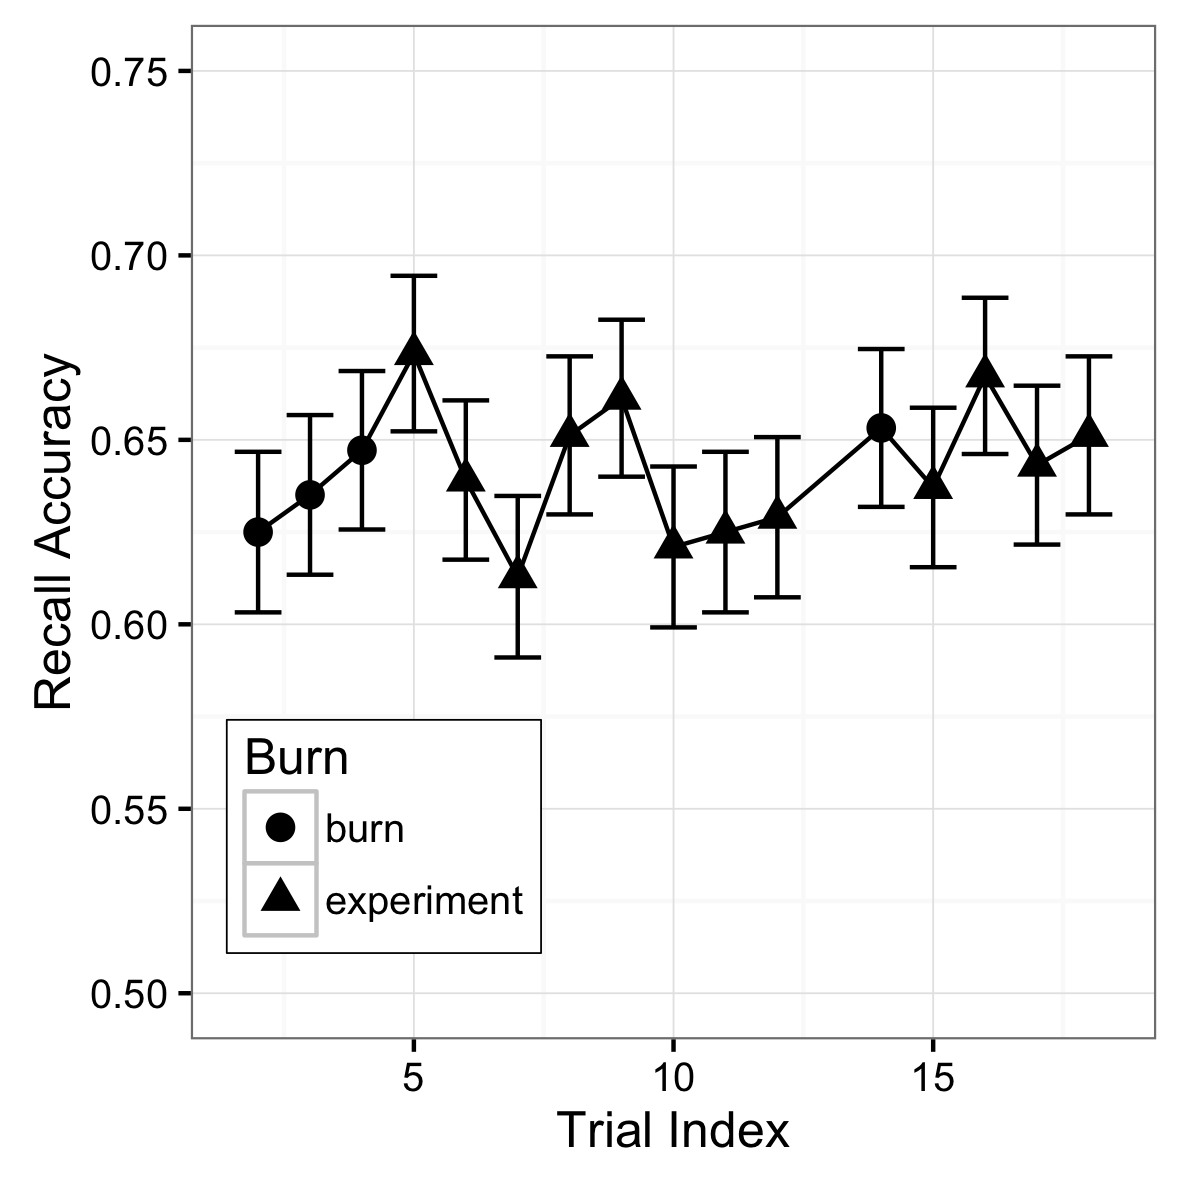
\includegraphics[width=.9\linewidth]{figures/conf2_stoIdxWburn.png}
\caption{Mean and standard error of each trial position with grand mean.}
\label{fig:conf2_stoIdx}
\end{minipage}
\end{figure}

\subsubsection{Confounding Effects}
The small difference in recall success depending on the story structure type (analogical vs. filler) was not replicated in experiment 2. Figure \ref{fig:conf2_conditionWburn} depicts the different recall accuracy for each condition. The ${\chi}^2$-test of independence did not show any significance (\textit{${\chi}^2$}( 2, \textit{N} = 7936) = 1.0419, \textit{p} = 0.59).

In contrast to experiment 1 and to my surprise, in experiment 2 no increased memory performance effect over trial index could be observed in a simple logistic regression (\textit{e}=0.001, \textit{z}(5950)=0.194, \textit{p}=0.846). Figure \ref{fig:conf2_stoIdx} shows the absence of any tendency in recall accuracy over trial index. Considering the differences between experiment 1 and 2, I can think of four reasons, why this finding from experiment 1 could not be replicated, which are listed first and then investigated.
First (a), there is no such effect in this experimental setting and the evidence in experiment 1 was obtained by chance. Second (b), the increased difficulty through the limited encoding time in experiment 2 introduced more variance, which could overshadow such a subtle effect. Third (c), the new burn-in phase (the first three trials in the beginning of experiment 2) took the wind out of the sails, meaning there is only an increase in recall performance over the very first few trials. And fourth (d), the samples differed regarding a certain parameter, which interacts with the trial index.

The last hypothesis (d) can be investigated regarding the three demographic variables that were recorded, which are age, gender and highest degree of education. The variables gender and highest degree of education both did not differ significantly between the two experiments, according to a ${\chi}^2$-test of independence (gender: \textit{${\chi}^2$}(2, \textit{N} = 147) = 0.923, \textit{p} = 0.63; education: \textit{${\chi}^2$}(2, \textit{N} = 147) = 3.19, \textit{p} = 0.20). A Welch's t-test between both sample's age distribution shows marginal significance (\textit{t}(147) = 1.81, \textit{p} = 0.073), indicating that the different age distributions might play a role in explaining differences between the two experiments. Age did not play a significant role when trying to predict overall recall accuracy controlling for experiment differences in linear regression (\textit{e} < 0.001, \textit{t}(144) = 0.182, \textit{p} = 0.856), but could still have an effect on the learning rate. \cite{Gagnon2005} and \cite{Turcotte2005} could find evidence for this claim, but in both those studies the investigated groups differed by about 50 years on average, but the difference of the means of our samples is less then 4 years. These arguments make this hypothesis (d) a rather unlikely reason for the absence of a trial index effect in experiment 2.

Despite the fact that we observed a trial index effect in experiment 1 even when the first trial position had a free parameter (model 6 in table \ref{table:main}), the novel burn-in phase can be seen as an extended version of what was measured by the "first" parameter. The influence of the first few trials and not just the first trial on the trial index effect should therefore be reassessed. This hypothesis (c) is opposed by the fact, that even when excluding the first three trials in experiment 1, there's still a strong trial index effect on recall success in a logistic regression analysis (\textit{e} = 0.029, z(9518) = 3.558, \textit{p} < 0.001), meaning that at least in experiment 1 the first three trials are not solely responsible for the trial index effect. Additionally, this hypothesis is also contradictory to the logistic regression including the data from burn-in trials in experiment 2, which also does not show a trial position effect (\textit{e} = 0.003, z(7936) = 0.626, \textit{p} = 0.532). This can also be seen in figure \ref{fig:conf2_stoIdx}.

Both Levene tests for homogeneity of variances, the one reported for stories (see Experiment 2: Material Assessment) and the one for participants (see Experiment 2: General Task Performance) showed an increased variance in experiment 2 due to increased task difficulty. This indicates an increased sensitivity regarding individual or story differences but has also introduced new variance, which could overshadow a trial index effect. This hypothesis (b), is also supported by the finding that neither an "after trick" nor a "first" position effect were detected in experiment 2, which could also be explained with increased noise. In experiment 1 a remarkable decrease in recall success after the trick story, as well as a greatly decreased recall performance at the first trial position could be observed. The logistic regression when controlling for trial index effects neither shows significance for after trick trials (\textit{e}=0.041, \textit{z}(7936) = 0.413, \textit{p} = 0.68), nor the first story position (\textit{e} = -0.065, \textit{z}(7936) = -0.624, \textit{p} = 0.533). In experiment 2 the first trials were part of the burn-in phase, but there is no reason to believe that these stories were less difficult, as was reported above. The concurrent absence of all three trial position effects indicate a systematic difference between experiment 1 and 2, which is likely to be a consequence of the increased difficulty due to the greatly reduced reading time.

Hypothesis one (a), that the results from experiment 1 were mere coincidence, can not be completely neglected, but given the alternative explanation for the absence of a trial index effect make it seem unlikely.

\begin{figure}
\begin{minipage}[t]{.5\textwidth}
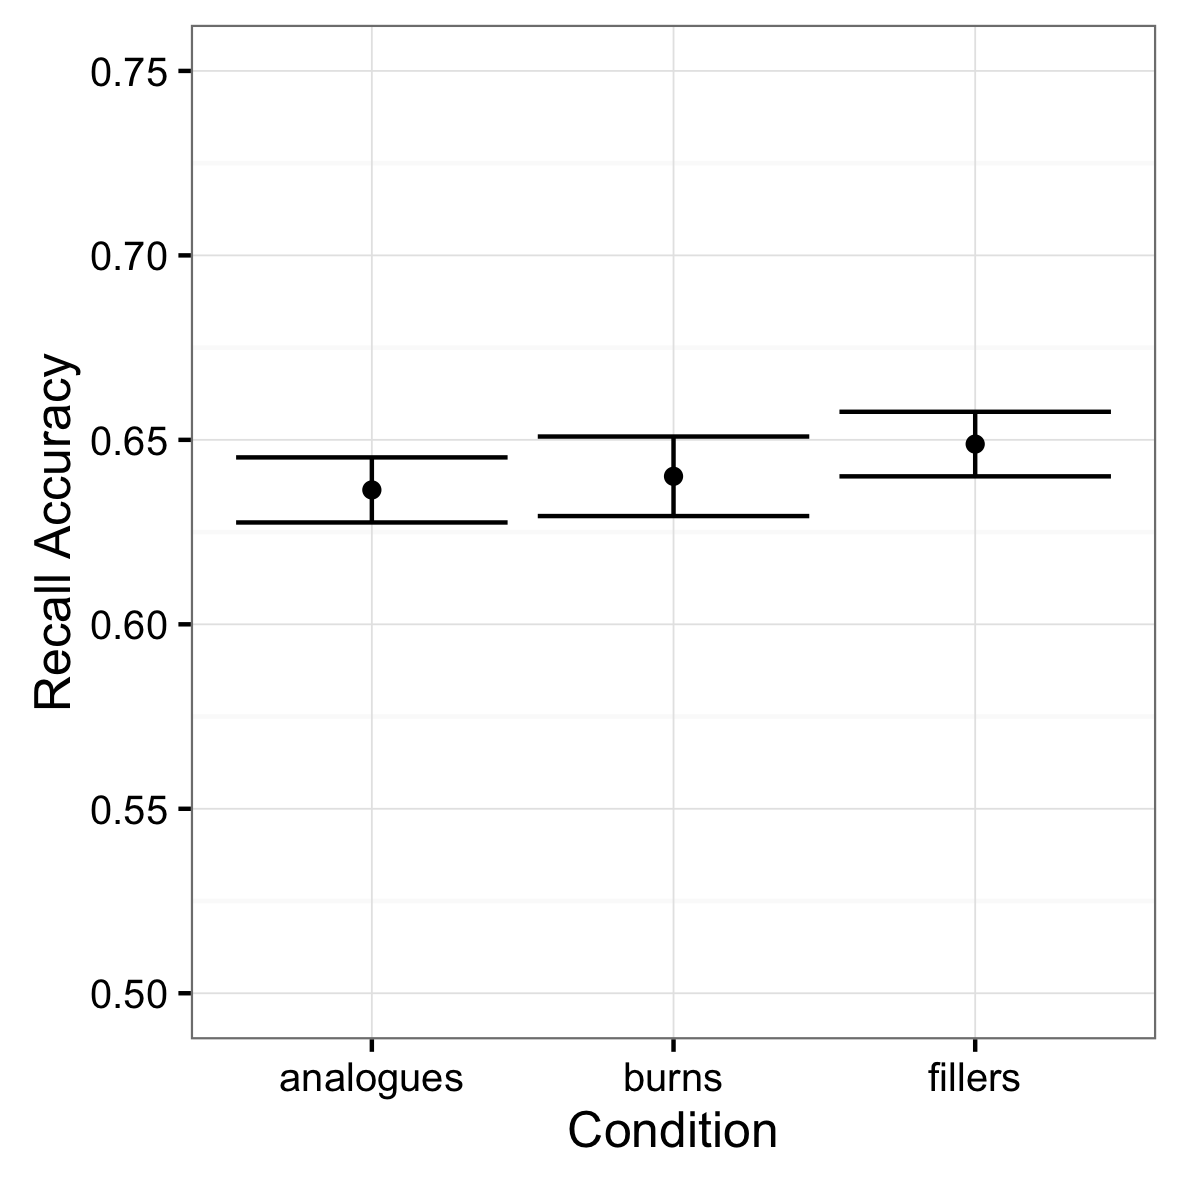
\includegraphics[width=.9\linewidth]{figures/conf2_conditionWburn.png}
\caption{Mean and standard error for each condition.}
\label{fig:conf2_conditionWburn}
\end{minipage}
\begin{minipage}[t]{.5\textwidth}
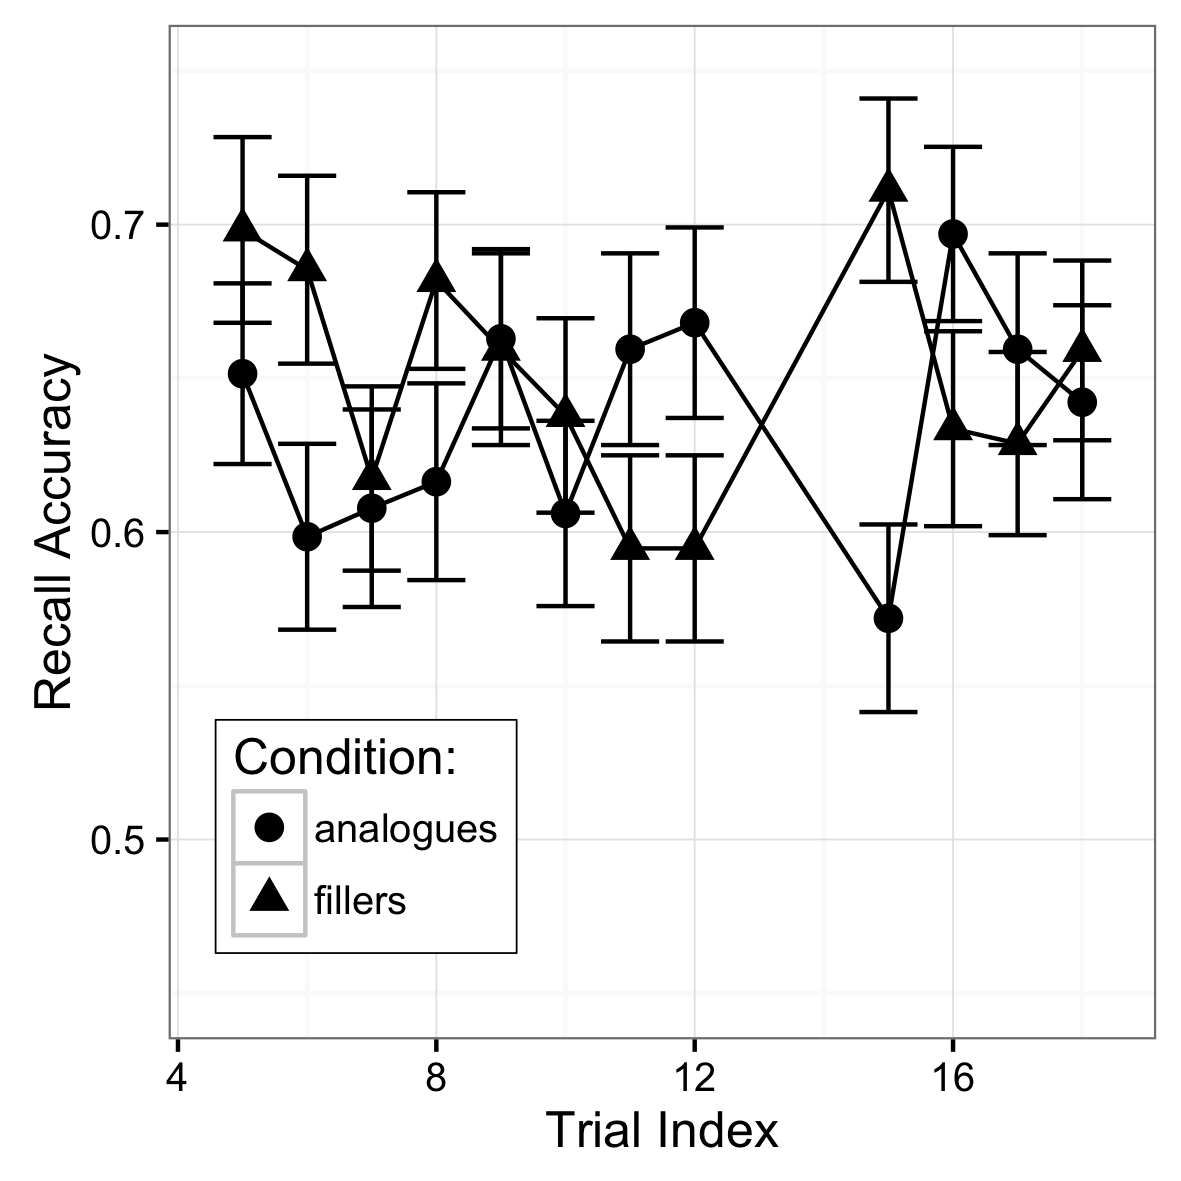
\includegraphics[width=.9\linewidth]{figures/main2.png}
\caption{Mean and standard error for each trial index and condition .}
\label{fig:main2}
\end{minipage}
\end{figure}


The other confounding effects like statement position and response type look very much like in experiment 1, although sometimes a little different accentuated.

\subsubsection{Main Effects}


% Table created by stargazer v.5.2 by Marek Hlavac, Harvard University. E-mail: hlavac at fas.harvard.edu
% Date and time: Fri, Aug 12, 2016 - 20:03:47
\begin{table}[!htbp] \centering
  \caption{}
  \label{table:main2}
  \small
  \renewcommand{\arraystretch}{0.6}
\begin{tabular}{@{\extracolsep{5pt}}lcccc}
\\[-1.8ex]\hline
\hline \\[-1.8ex]
 & \multicolumn{4}{c}{\textit{Dependent variable:}} \\
\cline{2-5}
\\[-1.8ex] & \multicolumn{4}{c}{Recall Sucess} \\
\\[-1.8ex] & (1) & (2) & (3) & (4)\\
\hline \\[-1.8ex]
 Trial Index & 0.009 & 0.008 & 0.008 & 0.008 \\
  & (0.030) & (0.031) & (0.030) & (0.031) \\
  & & & & \\
 Response Type Relation & $-$0.496$^{**}$ & $-$0.496$^{**}$ & $-$0.497$^{**}$ & $-$0.497$^{**}$ \\
  & (0.063) & (0.063) & (0.063) & (0.063) \\
  & & & & \\
 Statement Nr 2 & $-$0.323$^{**}$ & $-$0.323$^{**}$ & $-$0.323$^{**}$ & $-$0.323$^{**}$ \\
  & (0.085) & (0.083) & (0.084) & (0.084) \\
  & & & & \\
 Statement Nr 3 & 0.692$^{**}$ & 0.692$^{**}$ & 0.693$^{**}$ & 0.693$^{**}$ \\
  & (0.096) & (0.095) & (0.096) & (0.096) \\
  & & & & \\
 Primed &  & $-$0.003 &  & $-$0.003 \\
  &  & (0.061) &  & (0.061) \\
  & & & & \\
 Condition &  & 0.026 & 0.033 & 0.030 \\
  &  & (0.047) & (0.036) & (0.048) \\
  & & & & \\
 Primed:Condition &  & 0.013 &  &  \\
  &  & (0.061) &  &  \\
  & & & & \\
 Trial Index:Condition &  &  & $-$0.035 & $-$0.034 \\
  &  &  & (0.031) & (0.031) \\
  & & & & \\
 Condition:Primed &  &  &  & 0.005 \\
  &  &  &  & (0.061) \\
  & & & & \\
 Constant & 0.941$^{**}$ & 0.943$^{**}$ & 0.942$^{**}$ & 0.944$^{**}$ \\
  & (0.167) & (0.170) & (0.167) & (0.170) \\
  & & & & \\
\hline \\[-1.8ex]
Observations & 5,952 & 5,952 & 5,952 & 5,952 \\
Log Likelihood & $-$3,321.002 & $-$3,320.571 & $-$3,319.984 & $-$3,319.979 \\
Akaike Inf. Crit. & 6,656.004 & 6,661.143 & 6,657.968 & 6,661.958 \\
Bayesian Inf. Crit. & 6,702.844 & 6,728.058 & 6,718.191 & 6,735.564 \\
\hline
\hline \\[-1.8ex]
\textit{Note:}  & \multicolumn{4}{r}{\textsuperscript{o} p<0.1; * p<0.05; ** p<0.01; *** p<0.001} \\
\end{tabular}
\end{table}


Even though a trial index effect was not detected, there still could be an interaction with the story structure condition. An improved recall performance in the analogical condition could for example be overshadowed by a stable performance throughout the experiment in the filler condition, which could have resulted in not finding a trial index effect. Also, with the immediate repetition of the conditions, I introduced a binary variable I called "primed" in experiment 2, reflecting if the previous trial was from the same condition or not. "Primed" could show additional benefits in recall through immediate repetition of a story structure, similar to priming studies. Because I expect this effect only to appear in the analogical condition, I have to test the interaction while controlling for story index effects.

Table \ref{table:main2} shows an overview of calculated logistic crossed random effects models. Figure \ref{fig:main2} shows the recall accuracy for each trial index and condition, which shows no clear tendency of an interaction between condition and trial index. This is confirmed in the model 3 and 4 of table \ref{table:main2} where the interaction shows no significance. The primed effect shows no significance in the models 2 and 4 of the same table, which can also be seen in figure \ref{fig:main2b}. The standard errors are overlapping a lot.

\begin{figure}
\begin{minipage}[t]{.5\textwidth}
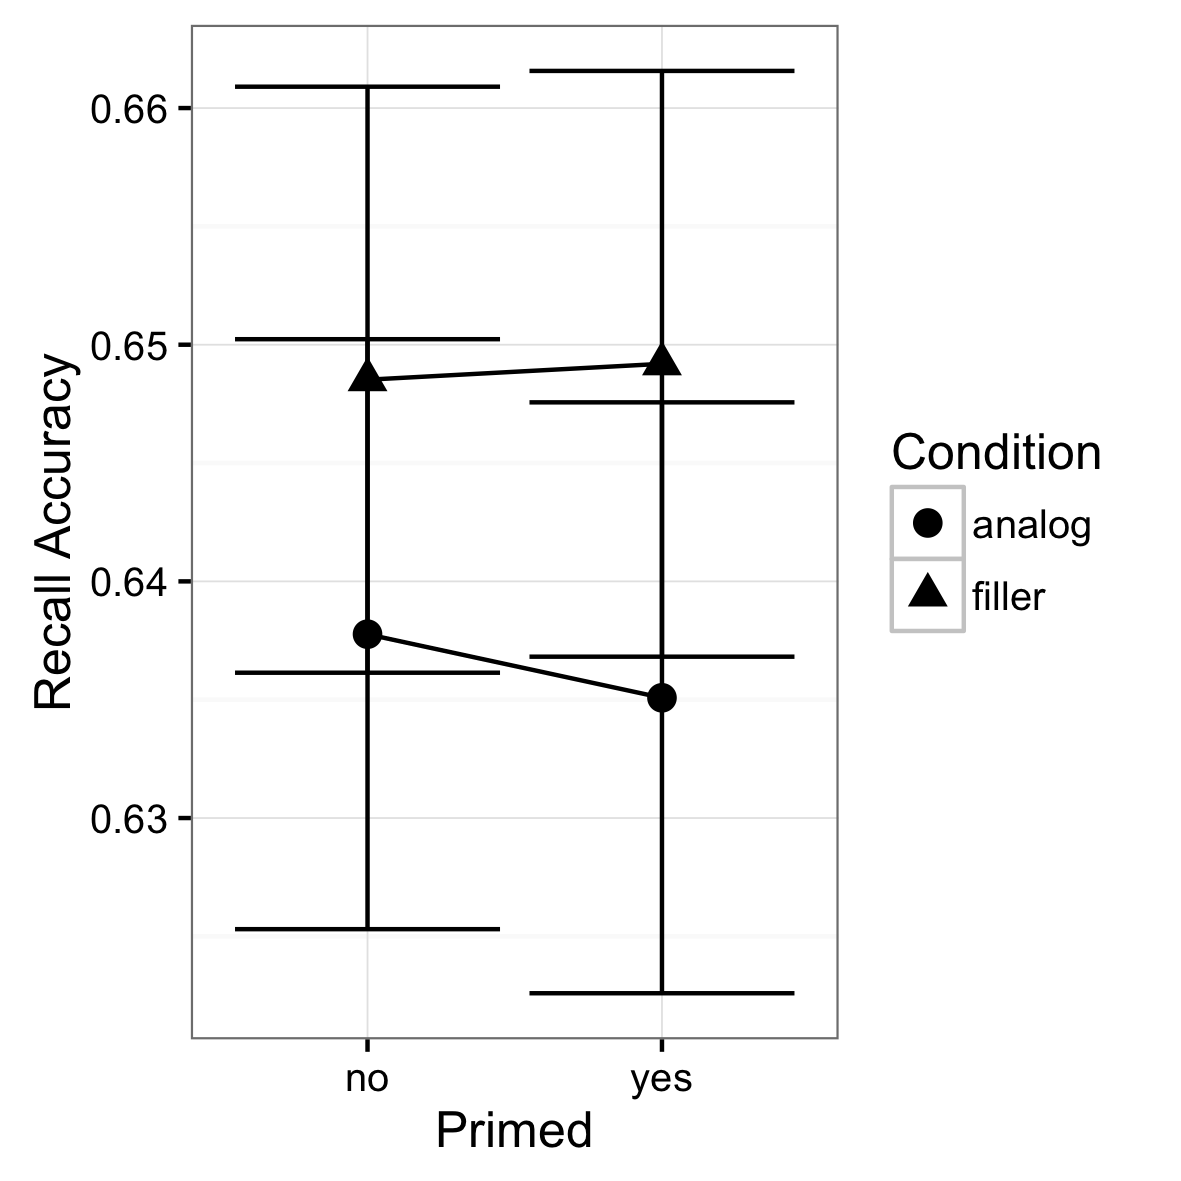
\includegraphics[width=.9\linewidth]{figures/main2b.png}
\caption{Mean and standard error for primed and condition.}
\label{fig:main2b}
\end{minipage}
\begin{minipage}[t]{.5\textwidth}
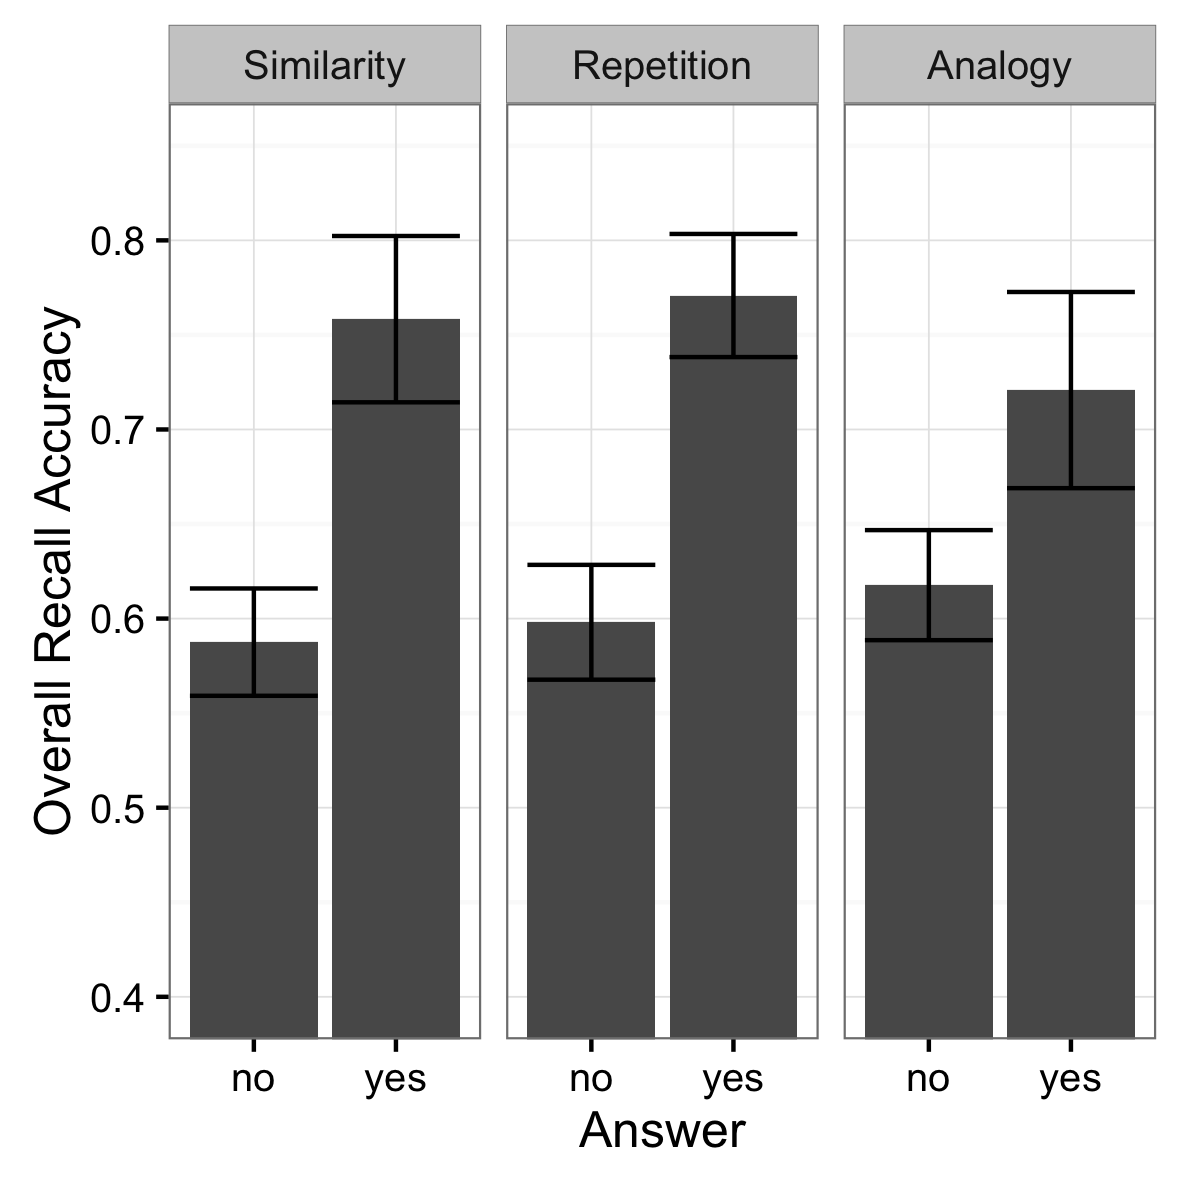
\includegraphics[width=.9\linewidth]{figures/fol2_answerXoverall.png}
\caption{Mean and standard error of subjects' recall accuracy for each follow-up question.}
\label{fig:fol2}
\end{minipage}
\end{figure}

I have already argued, that the increased task difficulty in the second experiment led to increased noise, which could have overshadowed the trial index effect. The same could be true for even weaker effects like the interaction with condition or the effect of primed and condition. Although in this case, I have less evidence that speaks for this explanation. The alternative explanation, that those interaction effects were obtained by chance in the first experiment seems more likely, than when arguing against chance for the trial index effect.


% Table created by stargazer v.5.2 by Marek Hlavac, Harvard University. E-mail: hlavac at fas.harvard.edu
% Date and time: Fri, Aug 12, 2016 - 20:57:15
\begin{table}[!htbp] \centering
  \caption{Regression Coefficients and Standard Errors in Parentheses}
  \label{table:fol2}
  \small
  \renewcommand{\arraystretch}{0.6}
\begin{tabular}{@{\extracolsep{5pt}}lccc}
\\[-1.8ex]\hline
\hline \\[-1.8ex]
 & \multicolumn{3}{c}{\textit{Linear Regression Models predicting Overall Recall Accuracy:}} \\
\cline{2-4}
\\[-1.8ex] & (1) & (2) & (3)\\
\hline \\[-1.8ex]
 Similarity & 0.171$^{**}$ &  &  \\
  & (0.051) &  &  \\
  & & & \\
 Repetition &  & 0.173$^{**}$ &  \\
  &  & (0.055) &  \\
  & & & \\
 Analogy &  &  & 0.103$^{o}$ \\
  &  &  & (0.059) \\
  & & & \\
 Constant & 0.588$^{**}$ & 0.598$^{**}$ & 0.618$^{**}$ \\
  & (0.029) & (0.028) & (0.029) \\
  & & & \\
\hline \\[-1.8ex]
Observations & 62 & 62 & 62 \\
R$^{2}$ & 0.157 & 0.141 & 0.048 \\
Adjusted R$^{2}$ & 0.143 & 0.127 & 0.032 \\
Residual Std. Error (df = 60) & 0.188 & 0.190 & 0.200 \\
F Statistic (df = 1; 60) & 11.177$^{**}$ & 9.835$^{**}$ & 3.030$^{o}$ \\
\hline
\hline \\[-1.8ex]
\textit{Note:}  & \multicolumn{3}{r}{\textsuperscript{o} p<0.1; * p<0.05; ** p<0.01; *** p<0.001} \\
\end{tabular}
\end{table}


\subsubsection{Post-Experiment Questionnaire}
The percentages of self-reported similarity detection between the stories were comparable to those of experiment 1. What differed though, was the effects of similarity detection on recall performance. Table \ref{table:fol2} shows an overview over three linear models predicting overall recall performance, one for each of the three follow-up questions (see appendix). Figure \ref{fig:fol2} shows the differences in recall performance with respect to similarity detection. It appears to be the case, that people that were aware of the certain similarities or repeating elements had higher recall accuracies than participants that reported to not have noted any differences. I can only speculate if this effect appeared due to an increase in task sensitivity regarding an individuals abilities.

\subsection{Conclusion}
In the second experiment most findings from the first experiment could not be replicated. Setting a limit of 3 seconds reading time per statement, which is less then half of the median participants used to read the statements in experiment 1, changed how trial index relates to recall performance and the interaction with story structure condition as well. Neither could the predicted effect of immediate repeated story structure be observed.

\newpage
\section{General Discussion}

% similarity and memory
% transfer ressources
% differences in syntax

The aim of this thesis was to investigate whether recall performance changes over repeated causal structures in analogical stories, building on previous research from relational priming and analogical reminding studies. By combining an established method from memory research with original story material, a novel experimental setting was developed to investigate this hypothesis and contribute to growing evidence that analogical transfer happens also unintentionally. It would for the first time indicate that unintentional analogical transfer can also rely on mere structural similarity. Weak evidence for this effect could be obtained in experiment 1, where I observed an interaction of story structure condition (analogical vs. filler) and trial index on the the 5\%-significance level. This effect could not be replicated in experiment 2, where the trial sequence was changed to a repeated story structure setting and limited reading time was introduced. Because various effects from experiment 1 concurrently could not be replicated in experiment 2, I argued that the most probable reason was the increased task difficulty through the limited encoding time.

\subsection{Limitations and Future Directions}
\subsubsection{Material}
Materials were constructed specifically for this experiment and not validated before using it in the experiments, neither regarding their structural nor surface similarity. I only tested different story lengths to find a suitable amount of statements per story. The argument therefore can be made, that the analogical stories did not actually share structural similarity, an assumption I made when building those stories. Also, I claim that our stories generally share no or only very few surface features. Through independent ratings by pairwise comparisons of stories, the subjective perceptions of those different kinds of similarities could at least be investigated.

\subsubsection{Processing Depth}
Another major concern regarding this experimental setup is: how well are participants integrating the information they were encoding? It is important to note this, because analogical stories only share abstract information. Therefore, an increased recall performance could only be observed, if the information is encoded on the required level of abstraction. The task they had to solve was pure recall and even though I asked the participants for the relations between two entities, I did not check how well the information was integrated and how deep it was processed. Participants could just as well have remembered the sequence of items and not integrate the information into more abstract representations. Evidence that this might be important can be seen in a study from \cite{Spellman2001}. They only detected a relational priming effect when they asked participants to pay attention and use the relation. Also it seems to be the case when comparing various relational priming studies, that the kind of task participants had to do, moderates the relational priming effect \citep{Popov2015}. In one study participants were asked if a word pair makes sense, which is also called a sensicality task \citep{Estes2006}. This task requires a higher degree of information integration than for example in a lexical decision task. It could be said that our task resembles more a lexical decision task than a sensicality task, a task  in terms of level of information integration.

One possibility to investigate this problem in future experiments, could be to add the passive relations as response options in the relation menu. For example, when a participant has read the statement "Bacteria A emits enzyme B" and then the correct response could be: "B" (name1), "is emitted by" (relation) and "A" (name2).
Through this, it probably might not be possible to force deeper information integration during encoding, but at least it could be measured and therefore controlled for. I assume that people with better integrated representations, should have less difficulties in responding to passive relations. This could become visible in lower decoding times or higher recall success rates.

To incentivize deeper processing of the stories, one could also think of an additional task. One option could be to ask the participants whether the conclusive statement makes sense, as was done in relational priming studies already \citep{Estes2006,Popov2015}. This could also be done while varying the sensicality of those conclusive statements. The bacteria story for example ("Bacteria A emits enzyme B", "Enzyme B dissolves the membrane of organ C.") could have two differing conclusive statements, i.e. "Organ C fails." (original) and "Organ C rules" (new and nonsensical). This addition would also be interesting to investigate, because the task would become better relatable to previous research in relational priming, when comparing reaction times of the sensicality judgement as was done before.

Individual differences regarding processing depth have not been accounted for in this thesis. According to the Theory Need for Cognition some people are generally more motivated to elaborate than others as kind of a personality trait \citep{Cacioppo1982,Cacioppo1996}. Therefore there also could be individual differences in our task regarding the abstraction of representations of the stories, which are not captured by the free parameters of the random effects. Individual differences could be measured with either the original NFC-questionnaire \citep{Cacioppo1982} or abbreviated forms of the NFC by \cite{Epstein1996} like REI-questionnaires, which are part of the cognitive-experiential self-theory. Controlling for individual differences can reduce the noise further in a regression analysis and therefore strengthen the statistical power of a very subtle effect.

\subsubsection{Task difficulty}
As I have discussed already, I think that task difficulty moderates the effect of repeated story structure on recall success. The fact that more than one of the observed effects in experiment 1 are absent in experiment 2  speak for this hypothesis (interaction condition with trial index, first position, after trick position). To strengthen this argument a manipulation of the encoding time with for example 2, 4 and 8 seconds encoding time could collect further evidence in favor of this hypothesis. Also a manipulation of story length to vary task difficulty could be considered.

\bibliography{_main}
\section{Appendix}
\subsection{Material Experiment 1}
\subsubsection{Instructions on CrowdFlower}
In this online experiment, participants will read a few, very short stories. After each story, participants are asked to recall the content of those stories by reconstructing its statements in the order of appearance.
It will take around 20 minutes. There will be a confirmation code handed out at the end. We'll grant you a bonus of 2\$ if we can see that you showed effort. You must be a native English speaker and use a recent version of Chrome, Safari or Firefox to take part in this experiment. Means to facilitate the task are not allowed. You can only take part, if you weren't part of the same experiment already (check here).
To start the experiment, please open the following link and carefully read the instructions.

\subsubsection{Follow-Up Questions}
\begin{enumerate}
  \item Did you notice similarities between the stories during the experiment (not now)?
  \item Did you notice repeating elements between the stories during the experiment?
  \item Did you notice any repeating analog/causal structure during the experiment?
\end{enumerate}

\subsubsection{Stories with Relation Response Options}
\begin{itemize}
\item Analog Stories:
\scriptsize
\begin{longtable}{p{.08\textwidth}p{.5\textwidth}p{.42\textwidth}}
\textbf{Title} & \textbf{Statement} &\textbf{Relation-Options}\\
Bacteria & Bacteria A emits enzyme B. & emits / expels / injects \\   & Enzyme B dissolves the membrane of organ C. & dissolves sth. of / disintegrates sth. of / disjoints sth. of \\   & Organ C fails. & fails / dies / is eliminated \\  & & \\ Crusader & Crusader group A bought weapon B. & bought / acquired / caught \\   & Weapon B breaches the fortification of town C. & breaches sth. of / breaks sth. of / passes sth. of \\   & Town C is invaded. & is invaded / is intruded / is infiltrated \\  & & \\ Hacker & Hacker A wrote computer code B. & wrote / invented / thought of \\   & Code B cracks the firewall of company C. & cracks sth. of / penetrates sth. of / catches sth. of \\   & Company C suffers a data loss. & suffers sth. / leaks sth. / tolerates sth. \\  & & \\ Lawyer & Lawyer A finds loophole B. & finds / detects / meets \\   & Loophole B bypasses contract of union C. & bypasses sth. of / overrides sth. of / bystands sth. of \\   & Union C loses a lawsuit. & loses sth. / forfeits sth. / files sth. \\  & & \\ Robber & Criminal A learns about security issue B. & learns about / finds out about / starts looking \\   & Security issue B suspends alarm system of museum C. & suspends sth. of / disrupts sth. of / inspects sth. of \\   & Museum C gets robbed. & gets robbed / endures loss / is hijacked \\  & & \\ Espionage & Country A trains spy B. & trains / instructs / creates \\   & Spy B is hired by Intelligence Agency of country C. & is hired by sth. of / is employed by sth. of / is fired by sth. of \\   & Country C has its secrets stolen. & has sth. stolen / has sth. poached / has sth. lost \\  & & \\ Fox & Fox A digs tunnel B. & digs / burrow / wants \\   & Tunnel B leads to coop of chicken C. & leads to sth. of / gets to sth. of / goes on sth. of \\   & Chicken C is devoured. & is devoured / is eaten / is missing \\  & & \\
\end{longtable}
\item \normalsize Filler Stories:
\scriptsize
\begin{longtable}{p{.08\textwidth}p{.5\textwidth}p{.42\textwidth}}
Meteo & Cloud A collects humidity over ocean B. & collects humidity over / is contained in / lies in front of \\   & Ocean B lies next to the beaches of area C. & lies next to / is located near / lies above \\   & Area C is fertile. & is fertile / is humid / is rich \\  & & \\ Fish & Fisher A cultivates sea grass B. & cultivates / grows / breeds \\   & Sea grass B is eaten by fish C. & is eaten by / is consumed by / is accepted by \\   & Fish C is captured. & is captured / is taken / is digested \\  & & \\ Farm & Farmer A bought machine B. & bought / purchased / borrowed \\   & Machine B can collect fruit of plant C. & can collect / garners / can compose \\   & Plant C are harvested automatically. & are harvested automatically / are reaped mechanically / are picked manually \\  & & \\ Mining & Mining company A has a lot of resource B. & has a lot of / is filled with / fills in for \\   & Resource B is sparse in country C. & is sparse in / is rarely found in / is sparked through \\   & Country C starts negotiating. & starts negotiating / starts brokering / starts trading \\  & & \\ Insect & Perfume A attracts insect B. & attracts / lures / smells \\   & Insect B attacks woman C. & attacks / assaults / approaches \\   & Woman C has an allergic reaction. & has an allergic reaction / reacts allergically / has a panic reaction \\  & & \\ Employee & Employee A is assigned to project B. & is assigned to / is referred to / is arranged to \\   & Project B supports agenda of manager C. & supports sth. of / emphasizes sth. of / destroys sth. of \\   & Manager C gets a promotion. & gets a promotion / gets an advancement / gets a bonus \\  & & \\ School & School girl A hits boy B. & hits / punches / touches \\   & Boy B reports to teacher C. & reports to / tells / goes to \\   & Teacher C calls parents. & calls parents / notifies parents / visits parents \\  & & \\
\end{longtable}
\end{itemize}


\subsubsection{Names}
List of randomly generated names for entities in stories. Names were generated using the free online tool dialectcreator.com:\newline
Titho / Ilres / Fozeh / Thygef / Dohod / Rove / Eshbu / Ottha / Thuha / Epnux / Evib / Potho / Ribi / Kawud / Avyth / Wehif / Uyim / Saly / Ohuy / Ezol / Eshov / Lyde / Huluw / Gena / Lenik / Upum / Hoyl / Afi / Yuxeh / Thisun / Ofes / Matmag / Vuloz / Puvi / Orok / Pishi / Thyra / Diaf / Hosen / Upno / Kewos / Hoap / Adjo / Olag / Uwit / Ebib / Rivo / Uhuy / Ihab / Vivaf / Felac / Newi / Ahow / Mabi / Owih / Rothuk / Napib / Assit / Eyem / Roze / Awiz / Zimob / Ifeh / Zidep / Wutoc / Molash / Ofpoz / Mawi / Afik / Reok / Yoges / Uvman / Vilux / Lothe / Inag / Goxos / Itbob / Mewep / Ewey / Meuf / Owmi / Upel / Eefar / Igoth / Olef / Ubug / Aid / Hadith / Enmob / Wecin / Turow / Paza / Hize / Gelyp / Idog / Vipal / Pide / Gabit / Zishu / Henu / Soav / Misug / Kesal / Dugoz / Pobat / Thusoth / Ohan / Romap / Zugew / Ena / Niem

\subsection{Material Experiment 2}
\subsubsection{Instructions on CrowdFlower}
In this online experiment, participants will be asked to read very short stories and recall its content after each story. The task is hard, don't expect to remember everything, but put in effort nonetheless. We will probe your attention. It will take around 15 to 20 minutes. There will be a confirmation code handed out at the end, but only if you pay attention to the task. You must be a native English speaker and use a recent version of Chrome, Safari or Firefox to take part in this experiment. We'll hand out a 1\$ bonus if you complete and pay attention. Also you can only take part if you weren't part of another experiment from us (check here).
To start the experiment, please open the following link and carefully read the instructions: Link

\subsubsection{Stories with Relation Response Options}
\begin{itemize}
\item Analog Stories:
\scriptsize
\begin{longtable}{p{.08\textwidth}p{.5\textwidth}p{.42\textwidth}}
\textbf{Title} & \textbf{Statement} &\textbf{Relation-Options}\\
Bacteria & Bacteria A emits enzyme B. & emits / expels / injects \\   & Enzyme B dissolves the membrane of organ C. & dissolves sth. of / disintegrates sth. of / disjoints sth. of \\   & Organ C fails. & fails / dies / is eliminated \\  & & \\ Crusader & Crusader group A buys weapon B. & buys / acquires / catches \\   & Weapon B breaches the fortification of town C. & breaches sth. of / breaks sth. of / passes sth. of \\   & Town C is invaded. & is invaded / is intruded / is infiltrated \\  & & \\ Hacker & Hacker A writes computer code B. & writes / invents / thinks of \\   & Code B cracks the firewall of company C. & cracks sth. of / penetrates sth. of / catches sth. of \\   & Company C suffers a data loss. & suffers sth. / leaks sth. / tolerates sth. \\  & & \\ Lawyer & Lawyer A finds loophole B. & finds / detects / meets \\   & Loophole B bypasses contract of union C. & bypasses sth. of / overrides sth. of / bystands sth. of \\   & Union C loses a lawsuit. & loses sth. / forfeits sth. / files sth. \\  & & \\ Robber & Criminal A learns about security issue B. & learns about / finds out about / starts looking \\   & Security issue B suspends alarm system of museum C. & suspends sth. of / disrupts sth. of / inspects sth. of \\   & Museum C gets robbed. & gets robbed / endures loss / is hijacked \\  & & \\ Fox & Fox A digs tunnel B. & digs / burrow / wants \\   & Tunnel B leads to coop of chicken C. & leads to sth. of / gets to sth. of / goes on sth. of \\   & Chicken C is devoured. & is devoured / is eaten / is missing \\  & & \\
\end{longtable}
\item \normalsize Filler Stories:
\scriptsize
\begin{longtable}{p{.08\textwidth}p{.5\textwidth}p{.42\textwidth}}
Storm & Storm A hits tree B. & hits / blows off / runs over \\   & Tree B falls on trail of route C. & falls on / drops on / is thrown on \\   & Route C is blocked. & is blocked / is jammed / is ruined \\  & & \\ Farm & Farmer A purchases machine B. & purchases / buys / borrows \\   & Machine B can collect fruit of plant C. & can collect / garners / can compose \\   & Plant C are harvested automatically. & are harvested automatically / are reaped mechanically / are picked manually \\  & & \\ Mining & Mining company A has a lot of resource B. & has a lot of / is filled with / fills in for \\   & Resource B is sparse in country C. & is sparse in / is rarely found in / is sparked through \\   & Country C starts negotiating. & starts negotiating / starts brokering / starts trading \\  & & \\ Pump & Plumber A installs pump B. & installs / builds / fixes \\   & Pump B sucks water from ground C. & sucks sth. from / transports sth. from / elevates sth. from \\   & Ground C dries up. & dries up / dehydrates / soakes up \\  & & \\ Employee & Employee A is assigned to project B. & is assigned to / is referred to / is arranged to \\   & Project B supports agenda of manager C. & supports sth. of / emphasizes sth. of / destroys sth. of \\   & Manager C gets a promotion. & gets a promotion / gets an advancement / gets a bonus \\  & & \\ Neighbor & Man A takes care of cat B. & takes care of / looks after / is feeding \\   & Cat B walks over the flowers of neighbor C & walks over sth. of / goes over sth. of / strays over to \\   & Neighbor C gets angry. & gets angry / becomes furious / gets aroused \\  & & \\
\end{longtable}
\item \normalsize Burn-In Stories:
\scriptsize
\begin{longtable}{p{.08\textwidth}p{.5\textwidth}p{.42\textwidth}}
Fish & Fisher A cultivates sea grass B. & cultivates / grows / breeds \\   & Sea grass B is eaten by fish C. & is eaten by / is consumed by / is accepted by \\   & Fish C is captured. & is captured / is taken / is digested \\  & & \\ School & School girl A beats boy B. & beats / punches / touches \\   & Boy B reports to teacher C. & reports to / tells / goes to \\   & Teacher C calls parents. & calls parents / notifies parents / visits parents \\  & & \\ Insect & Perfume A attracts insect B. & attracts / lures / smells \\   & Insect B attacks woman C. & attacks / assaults / approaches \\   & Woman C has an allergic reaction. & has an allergic reaction / needs medical support / has a panic reaction \\  & & \\ Meteo & Cloud A collects humidity over ocean B. & collects humidity over / is contained in / lies in front of \\   & Ocean B lies next to the beaches of area C. & lies next to / is located near / lies above \\   & Area C is fertile. & is fertile / is humid / is rich \\  & & \\
\end{longtable}
\end{itemize}


\includepdf{selbstaendigkeit}
\end{document}
